\documentclass[a4paper]{article}

\setlength{\parindent}{0pt}
\setlength{\parskip}{1em}

\pagestyle{headings}

\usepackage{amssymb}
\usepackage{amsmath}
\usepackage{amsthm}
\usepackage{mathtools}
\usepackage{graphicx}
\usepackage{hyperref}
\usepackage{color}
\usepackage{microtype}
\usepackage{tikz}
\usepackage{pgfplots}
\usepackage{pgfplotstable}

\newcommand{\N}{\mathbb{N}}
\newcommand{\Q}{\mathbb{Q}}
\newcommand{\Z}{\mathbb{Z}}
\newcommand{\R}{\mathbb{R}}
\newcommand{\C}{\mathbb{C}}
\newcommand{\D}{\mathcal{D}}
\renewcommand{\S}{\mathcal{S}}
\renewcommand{\P}{\mathbb{P}}
\newcommand{\F}{\mathbb{F}}
\newcommand{\E}{\mathbb{E}}
\newcommand{\bra}{\langle}
\newcommand{\ket}{\rangle}


\graphicspath{{Image/}}

\hypersetup{
    colorlinks=true,
    linktoc=all,
    linkcolor=blue
}

\theoremstyle{definition}
\newtheorem*{axiom}{Axiom}
\newtheorem*{claim}{Claim}
\newtheorem*{conv}{Convention}
\newtheorem*{coro}{Corollary}
\newtheorem*{defi}{Definition}
\newtheorem*{eg}{Example}
\newtheorem*{lemma}{Lemma}
\newtheorem*{notation}{Notation}
\newtheorem*{prob}{Problem}
\newtheorem*{post}{Postulate}
\newtheorem*{prop}{Proposition}
\newtheorem*{rem}{Remark}
\newtheorem*{thm}{Theorem}

\DeclareMathOperator{\vdiv}{div}
\DeclareMathOperator{\grad}{grad}
\DeclareMathOperator{\curl}{curl}
\DeclareMathOperator{\Ann}{Ann}
\DeclareMathOperator{\Fit}{Fit}
\DeclareMathOperator{\Diag}{Diag}
\DeclareMathOperator{\tr}{tr}
\DeclareMathOperator{\im}{im}
\DeclareMathOperator{\Mat}{Mat}
\DeclareMathOperator{\Log}{Log}
\DeclareMathOperator{\Isom}{Isom}
\DeclareMathOperator{\Mesh}{Mesh}
\DeclareMathOperator{\Sym}{Sym}
\DeclareMathOperator{\Aut}{Aut}
\DeclareMathOperator{\cosech}{cosech}
\DeclareMathOperator{\Card}{Card}
\DeclareMathOperator{\Gal}{Gal}


\setcounter{section}{-1}

\begin{document}

\title{Coding and Cryptography}

\maketitle

\newpage

\tableofcontents

\newpage

\section{Miscellaneous}

132

\newpage

\section{Introduction to communication channels and coding}
For example, given a message $M = "Call me!"$ which we wish to send by email. We first encode t as binary strings using ASCII. So $f(C) = 1000011$, $f(a) = 1100001$, $f^*(M) = 1000011 1100001 ... 0100001$. 

The message goes from the source to the receiver after encoded by the source and decoded by the receiver via a channel, where errors could occur. The basic problem is, given a source and a channel (described probabilistically, we aim to design an encoder and a decoder in order to transmit information economically, reliably, and preserving privacy (secretly).

Some examples of each aspect:\\
\emph{economcically}: Morse code, where common letters have shorter codewords;\\
\emph{reliability}: every book has an ISBN of form $a_1...a_{10}$ where $a_i \in \{0,1,...,9\}$ for $1 \leq i \leq 9$ and $a_{10} \in \{0,1,...,9,X\}$, s.t. $10 a_1 + 9a_2+...+a_{10} \equiv 0 \pmod 11$, where we treat $X$ as 10. In this way errors can be detected, although not corrected. There is another version of ISBN which is 13 digit;\\
\emph{preserve privacy} RSA.

A communication channel takes letters from an input alphabet $\Sigma_1 = \{a_1,...,a_r\}$ and emits letters from an output alphabet $\Sigma_2 = \{b_1,...,b_s\}$.

A channel is determined by the probabilities $P(y_1,...,y_k$ received$|x_1,...,x_k$ sent$)$.

\begin{defi}
A \emph{discrete memoryless channel}(DMC) s a channel for which $P_{ij} = P(b_j$ received$|a_i$ sent$)$ is the same each time the channel is used, and is independent of all past and future. The channel matrix is the $r \times s$ matrix with entrices $p_{ij}$. Note the rows sum to $1$.
\end{defi}

\begin{eg} (Binary Symmetric Channel, BSC)\\
BSC has $\Sigma_1 = \Sigma_2 = \{0,1\}$, $0 \leq p \leq 1$. It has channel matrix ${{1-p \ p} \choose {p \ 1-p}}$, i.e. $p$ is the probability symbol is mistransmitted.
\end{eg}

\begin{eg} (Binary Erasure Channel)\\
$\Sigma_1 = \{0,1\}$, $\Sigma_2 = \{0,1,*\}$, $0 \leq p \leq 1$. Then the channel matrix is ${{1-p \ p \ 0} \choose {0 \ p \ 1-p}}$, i.e. $p$ is the probability that a synbol can't be read.
\end{eg}

Informal definition: A channel's capacity is the highest rate at which information can be reliably transimitted over the channel. Here rate means the units of information per unit tme (we want that high), and reliably means arbitrarily small error probability.

There are 3 sections:\\
1) Noiseless coding (data compression);\\
2) Error control codes;\\
3) Cryptography.

\subsection{Noiseless coding}
\begin{notation}
For $\Sigma$ an alphabet that $\Sigma^* = \bigcup_{n \geq 0} \Sigma^n$ be th set of all finite strings of elements of $\Sigma$.
\end{notation}

If $x=x_1...x_r$, $y=y_1...y_s$ are strings from $\Sigma$, write $xy$ for the concatenation $x_1...x_ry_1...y_s$. Further, $|x_1...x_ry_1...y_s| = r+s$ the length of string.

\begin{defi}
Let $\Sigma_1,\Sigma_2$ be two alphabets. A \emph{code} is a function $f:\Sigma_1 \to \Sigma_2^*$. The strings $f(x)$ for $x \in E$ are called \emph{codewords}.
\end{defi}

\begin{eg} (Greek five code)\\
$\Sigma_1 = \{\alpha,\beta,...,\omega\}$ (24 letters); $\Sigma_2 = \{1,2,3,4,5\}$ (more used). Now let $\alpha \to 11, \beta \to 12, ...,\omega \to 54$.
\end{eg}

\begin{eg}
$\Sigma_1 = \{$all words in the dictionary$\}$. =,$\Sigma_2 = \{A,B,...,space\}$. Then $f=$'spell the word and a space.'
\end{eg}

We sent a message $x_1,...,x_n \in \Sigma^*_1$ as $f(x_1)f(x_2)...f(x_n) \in \Sigma_2^*$, i.e. extend $f$ to $f^* : \Sigma_1^* \to \Sigma_2^*$.

\begin{defi}
A code $f$ is \emph{decipherable} if $f^*$ is injective, i.e. every string from $\Sigma_2$ arises from at most one message.
\end{defi}

Note that $f$ being injective is not enough. See this example:

\begin{eg}
$\Sigma_1 = \{1,2,3,4\}$, $\Sigma_2 = \{0,1\}$, $f(1) = 0$, $f(2) = 1$, $f(3) = 00$, $f(4) = 01$. Then $f$ is injective, but $f^*(312) = 0001 = f^*(114)$ so $f^*$ is not decipherable.
\end{eg}

\begin{notation}
If $|\Sigma_1| = m$, $|\Sigma_2| = a$, then we say $f$ is an $a$-ary code of size $m$ (in particular, if $a=2$ we use the word binary).
\end{notation}

Our aim is to construct decipherable codes with short word lengths.

Provided $f:\Sigma_1 \to \Sigma^*_2$ is injective, the following codes are always decipherable:\\
(1) A \emph{Block code} is a code with all codewords of the same length (eg Greek fire code);\\
(2) In a \emph{comma code} we reserve one letter from $\Sigma_2$ that is only used to signal the end of the codeword (example 2);\\
(3) A \emph{prefix-free} code is a code where no codeword is a prefix of another (If $x,y \in \Sigma^*_2$, $x$ is a prefix of $y$ if $y=xz$ for some $z \in \Sigma^*_2$).

\begin{rem}
(1) and (2) are special cases of (3).
\end{rem}

Prefix-free codes are also known as \emph{instantaneous codes} (i.e. a word can be recognised as soon as its complete), or \emph{self-punctuating codes}.

\begin{thm} (1.1, Kraft's inequality)\\
Let $\Sigma_1| = m$, $\Sigma_2| = a$. A prefix-free code $f:\Sigma_1 \to \Sigma_2^*$ with word lengths $s_1,...,s_m$ exist iff $$\sum_{i=1}^m a^{-s_i} \leq 1$$
\begin{proof}
First we prove forward implication. Consider an infinite tree where each has a descendents, labelled by the elements of $\Sigma_2$. Each codeword corresponds to a node, the path from the root to this node spelling at the codeword. Assuming $f$ is prefix-free, no codeword is the ancestor of any other. Now view the tree as a network with water being pumped in at constant rate and divding the flow equally at each node. The total amount of water we can extract at the codewords is $\sum_{i=1}^m a^{-s_i}$ which is therefore $\leq 1$.

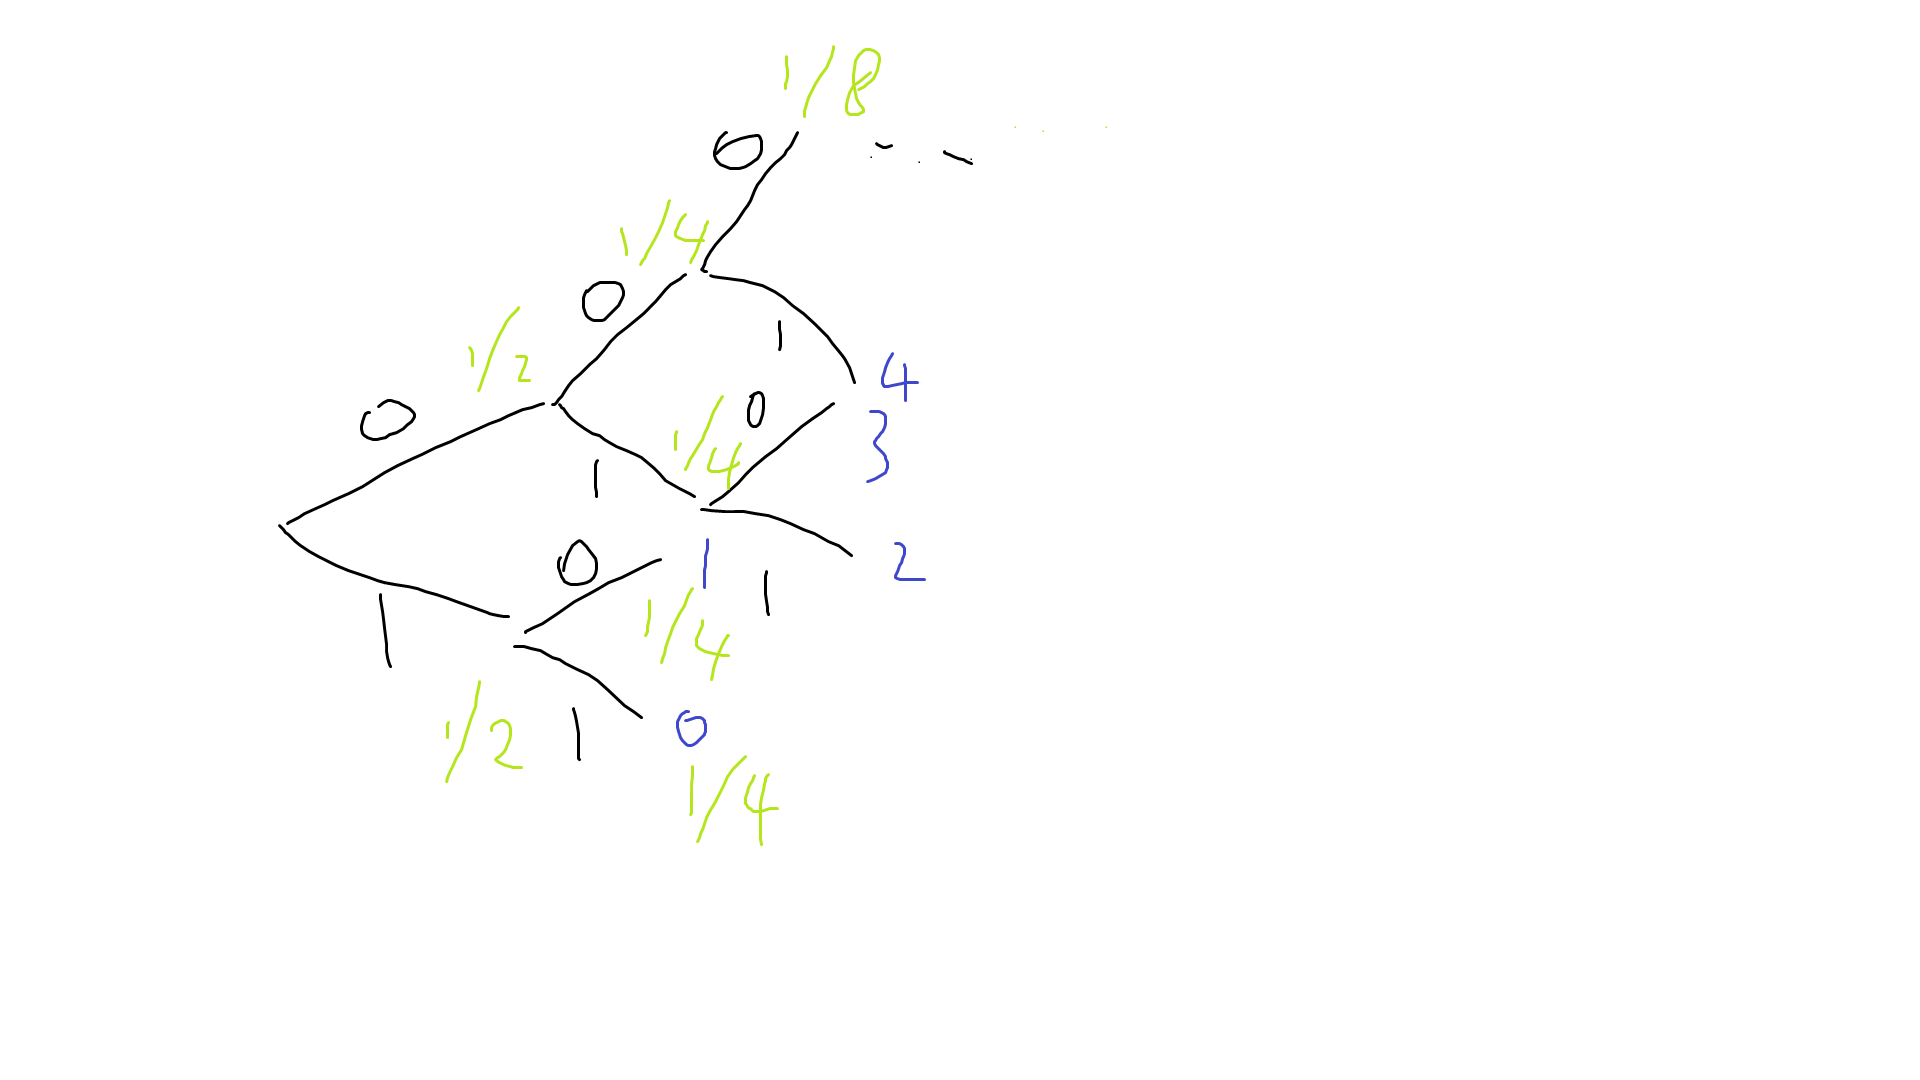
\includegraphics[scale=0.5]{image/CC_01.png}

Conversely, suppose we can construct a prefix-free code with word lengths $s_1,...,s_m$ , wlog $s_1 \leq s_2 \leq ... \leq s_m$. We pick codewords of lengths $s_1,...,$ sequentially ensuring previous codewords are not prefixes. Suppose there is no valid choice for the $r^{th}$ codeword. The constructing the tree as above gives $\sum_{i=1}^{r-1} a^{-s_i} = 1$, contradicting our assumption. So we can construct a prefix-free code.
\end{proof}
\end{thm}

\begin{thm} (1.2, Mcmillan)\\
Every decipherable code satisfies Kraft's inequality.
\begin{proof} (Karush)\\
Let $f:\Sigma_1 \to \Sigma_2^*$ be a decipherable code with word lengths $s_1,...,s_m$, let $s = \max_{1 \leq i \leq m} s_i$. Let $r \in \N$, $$(\sum_{i=1}^m a^{-s_i})^r = \sum_{b = 1}^{rs} b_i a^{-l}$$ where $b_i$ is the number of ways of choosing $r$ codewords of toatl length $l$. $f$ decipherable implies that $b_l \leq |\Sigma_2|^l = a^l$. Thus $(\sum_{i=1}^m a^{-s_i})^r \leq \sum_{l=1}^{rs} a^l a^{-l} = rs$, so $\sum_{i=1}^m a^{-s_i} \leq (rs^{1/r}) \to 1$ as $r \to \infty$. So $\sum_{i=1}^m a^{-s_i} \leq 1$.
\end{proof}
\end{thm}

So we have a corollary: a decipherable code with prescribed word lengths exist iff there exists a prefix-free code with the same word lengths.

So we can restrict our attention to prefix-free codes.

\subsection{Mathematical entropy}
Entropy is a measure of 'randomness' or 'certainty'. Consider a random variable $X$ taking values $x_1,...,x_n$ with probability $p_1,...,p_n$ ($\sum p_i = 1$, $0 \leq p_i \leq 1$). The entropy $H(x)$ is roughly speaking the expected number of tosses of a fair coin needed to simulate $X$ (or the expected number of yes/no questions we need to ask in order to establish the value of $X$).

\begin{eg}
Suppose $p_1 = p_2 = p_3 = p_4 = \frac{1}{4}$. We identify $\{x_1,...,x_4\}$ with $\{HH,HT,TH,TT\}$, so $H(x) = 2$.
\end{eg}

\begin{eg}
$(p_1,p_2,p_3,p_4) = (1/2,1/4,1/8,1/8)$. Then $H(x) = 1/2+1/4 \times 2 + 1/8 \times 3 + 1/8 \times 3=7/4$. So the entropy here is smaller.

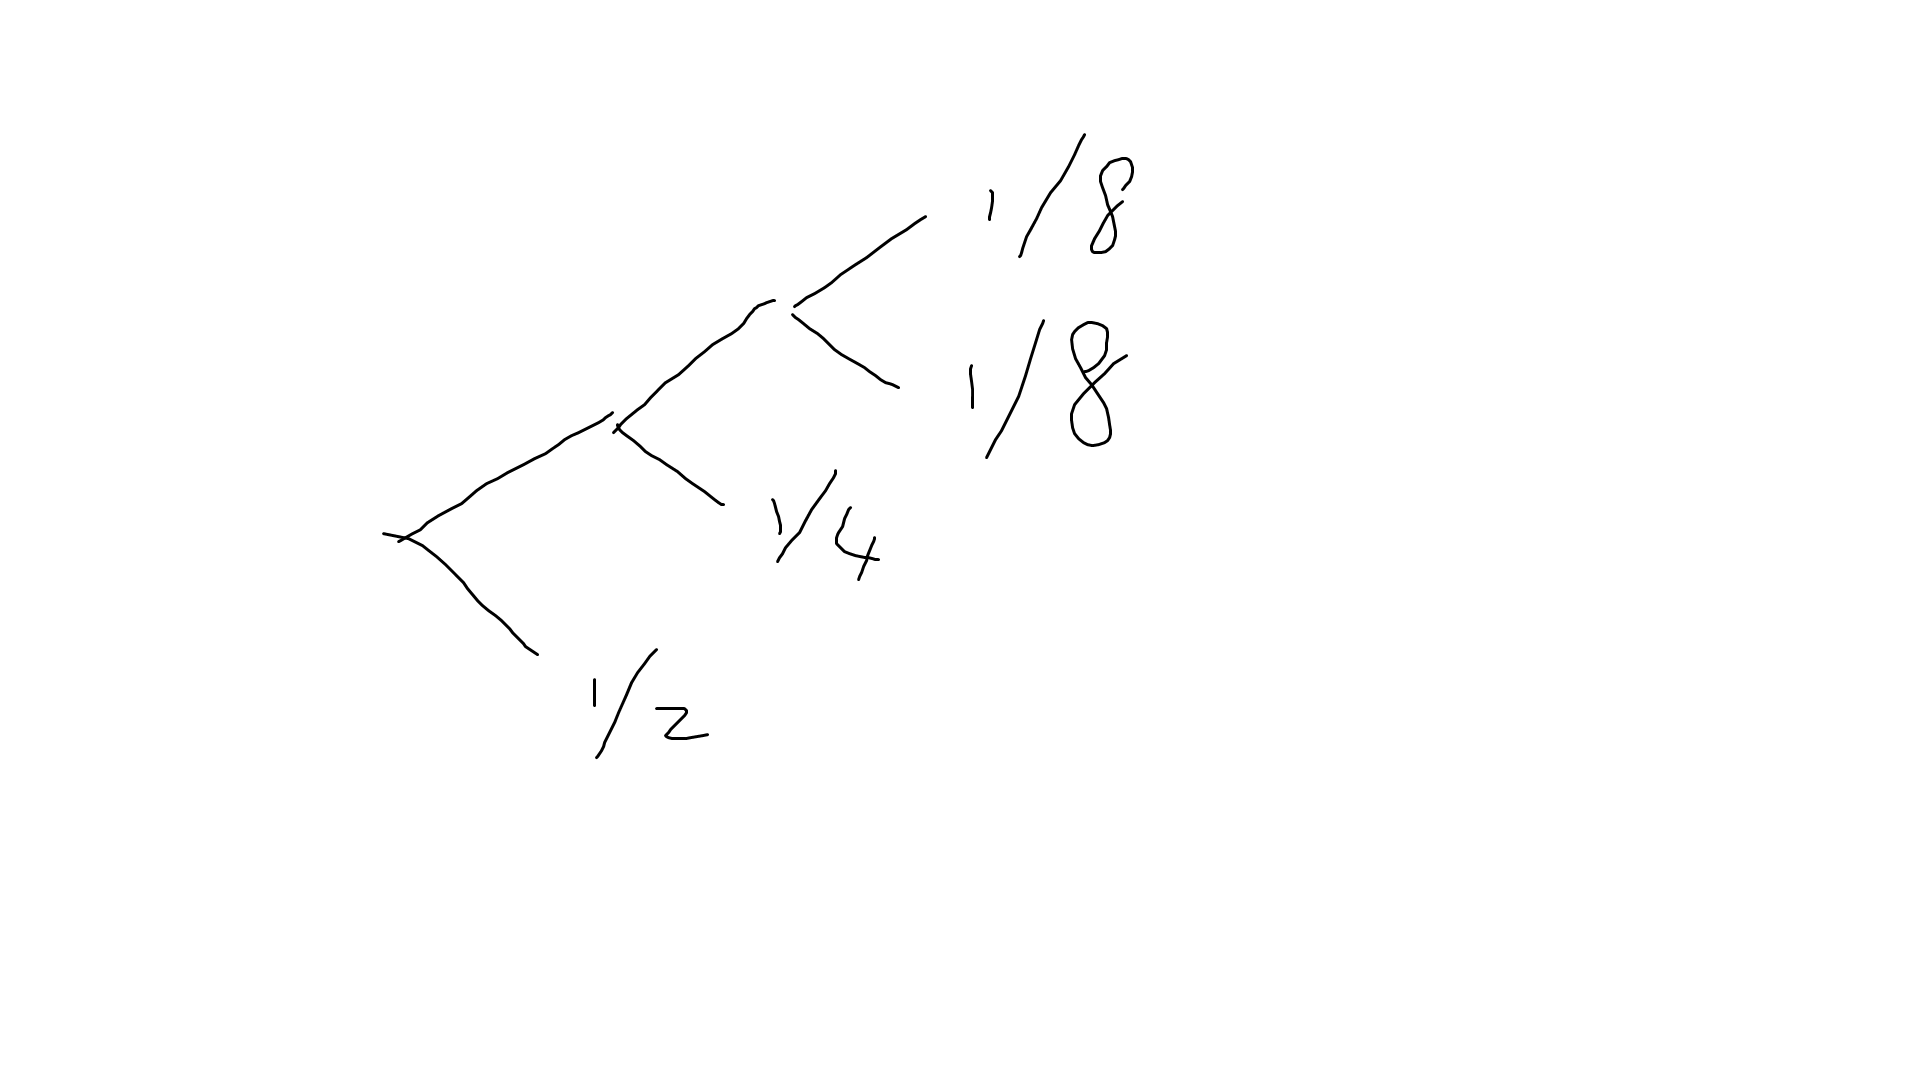
\includegraphics[scale=0.5]{image/CC_02.png}
\end{eg}

So in some sense, there is more randomness in the first example than the second.

\begin{defi} (Entropy)\\
The entropy of $X$, $$H(X) = H(p_1,...,p_n) = -\sum_{i=1}^n p_i \log p_i$$ where, as most of the time in this course, $\log = \log_2$.
\end{defi}

\begin{rem}
(1) If $p_i = 0$, we define $p_i \log p_i = 0$;\\
(2) $H(X) \geq 0$.
\end{rem}

\begin{eg} (3)\\
We toss a biased coin with $\P($heads$) = p$. Write $H(p) = H(p,1-p) = -p\log p - (1-p)\log(1-p)$. If $p=0$ or $1$, the outcome is certain and so entropy is $0$. Entropy is maximal where $p=1/2$ (check), a fair coin.

Note the entropy can also be viewed as the expected value of the information of $X$, where information is given by $I(X=x) = -\log \P(X=x)$. For example, if a coin always lands heads, we gain on information from tossing the coin.\\
This entropy is the average amount of information conveyed by a random variable $X$.
\end{eg}

\begin{lemma} (1.3, Gibbs' inequality)\\
Let $p_1,...,p_n$ and $q_1,...,q_n$ be probability distributions. Then $-\sum p_i \log p_i \leq -\sum p_i \log q_i$, with equality iff $p_i = q_i$.
\begin{proof}
It supplies to prove the inequality with $\log$ replaced by $\ln$. Note $\ln x \leq x-1$ with equality iff $x=1$. Let $I = \{1 \leq i \leq n: p_i \neq 0\}$. Then $\ln \frac{q_i}{p_i} \leq \frac{q_i}{p_i}-1$ $\forall i \in I$. So $\sum_{i \in I} p_i \ln \frac{q_i}{p_i} \leq \sum q_i - \underbrace{\sum p_i}_{=1} \leq 0$. Rearranging we get $-\sum_{i \in I} p_i \ln p_i \leq -\sum_{i \in I} p_i \ln q_i$, so $-\sum_{i=1}^n p_i \ln p_i \leq -\sum_{i=1}^n p_i \ln q_i$. If equality holds then $\frac{q_i}{p_i} = 1$ $\forall i \in I$, so $\sum_{i \in I} q_i = 1$ $\implies p_i = q_i$ for $1 \leq i \leq n$.
\end{proof}
\end{lemma}

\begin{coro}
$H(p_1,...,p_n) \leq \log n$ with equality iff $p_1 = p_2 = ... = p_n =\frac{1}{n}$.
\begin{proof}
Take $q_1=q_2=...=q_n = \frac{1}{n}$ in previous lemma.
\end{proof}
\end{coro}

Two alphabets $\Sigma_1,\Sigma_2$ with $|\Sigma_1| =m$, $|\Sigma_2| = a$ ($m \geq 2, a \geq 2$). We model the source as a sequence of random variables $X_1,X_2,...$ taking values in $\Sigma_1$.

\begin{defi}
A \emph{Bernoulli} or \emph{memoryless} source is a sequence of independently, identically distributed random variables, i.e. for each $\mu \in \Sigma_i$, the probability of $X_i = \mu$ is independent of $i$ and independent of all past and future symbols emitted. Thus $$\P(X_1=x_1,...,X_k = x_k) = \prod_{i=1}^k \P(X_i = x_i)$$

Let $\Sigma_1 =\{\mu_1,...,\mu_n\}$, $p_i = \P(X =\mu_i)$ and assume $p_i > 0$. The \emph{expected word length} of a code $f:\Sigma_1 \to \Sigma^*_2$ with word lengths $s_1,...,s_m$ is $E(S) = \sum_{i=1}^m p_i s_i$.
\end{defi}

\begin{defi}
A code $f:\Sigma_1 \to \Sigma^*_2$ is \emph{optimal} if it has the shortest possible expected word length among decipherable code.
\end{defi}

\begin{thm} (1.4, Shannon's Noiseless Coding theorem)\\
The minimum expected word length of a decipherable code $f:\Sigma_1\to \Sigma^*_2$ satisfies $$\frac{H(x)}{\log a} \leq E(S) < \frac{H(X)}{\log a} + 1$$
\begin{proof}
The lower bound is given by combining Gibbs and Kraft inequalities. Let $q_i = \frac{a^{-s_i}}{c}$ where $c = \sum a^{-s_i} \leq 1$ by Kraft's inequality. Note $\sum q_i = 1$. Now 
\begin{equation*}
\begin{aligned}
H(X) = -\sum p_i \log p_i &\leq -\sum_i p_i \log q_i \\
&= \sum_i p_i (s_i \log a + \log c)\\
&= (\sum_i p_i s_i) \log a + \log c\\
&\leq E(s) \log a
\end{aligned}
\end{equation*}
We get equality if and only if $p_i = a^{-s_i}$ for some integers $s_i$.

For the upper bound, put $s_i = \lceil -\log_a p_i \rceil$. We have $\log_a p_i \leq s_i < -\log_a p_i +1$, so $a^{-s_i} \leq p_i \implies \sum a^{-s_i} \leq \sum p_i \leq 1$. So by theorem (1.), there exists a prefix-free code with word lengths $s_1,...,s_m$.\\
Also,
\begin{equation*}
\begin{aligned}
E(S) &= \sum p_i s_i\\
&< \sum p_i (-\log_a p_i + 1)\\
&= \frac{H(X)}{\log a} + 1
\end{aligned}
\end{equation*}
\end{proof}
\end{thm}

\begin{rem}
The lower bound holds for all decipherable codes.
\end{rem}

Shannon-Fano Coding (as in Goldie $\&$ Pinch):\\
This follows from the proof above. Set $s_i = \lceil -\log_a p_i\rceil$ and construct a prefix-free code with word lengths $s_1,...,s_m$ by taking the $s_i$ in increasing order ensuring that previous codewords are not prefixes. The Kraft inequality ensures there is enough room.

\begin{eg}
$\mu_1,...,\mu_5$ emitted with probabilities $0.4,0.2,0.2,0.1,0.1$. We try to construct Shannon-Famo code (with $a=2$, $\Sigma_2 = \{0,1\}$):
\begin{equation*}
\begin{aligned}
\begin{matrix}
p_i & \lceil -\log p_i\rceil & \text{code}\\
0.4 & 2 & 00\\
0.2 & 3 & 010\\
0.2 & 3 & 100\\
0.1 & 4 & 1100\\
0.1 & 4 & 1110
\end{matrix}
\end{aligned}
\end{equation*}
The expected word length is $2 \times 0.4 + 3 \times 0.2 + 3 \times 0.2 + 4 \times 0.1 + 4 \times 0.1 = 2.8$.\\
As a comparison, $H(X) \approx 2.12$, which is consistent with our previous inequality.
\end{eg}

\begin{defi} (Huffman coding)\\
For simplicity we take $a=2$. Let $\Sigma_1 = \{\mu_1,...,\mu_m\}$, $p_i = \P(X=\mu_i)$. WLOG $p_1 \geq p_2 \geq ... \geq p_m$.  Huffman coding is defined inductively:\\
If $m=2$, assign codewords $0$ and $1$;\\
If $m>2$, find a Huffman coding in the case of meesages $\mu_1,\mu_2,...,\nu$ with probaiblities $p_1,p_2,...,p_{m-1}+p_m$; append $0$ (1 respectively) to the codeword for $\nu$ tove a codeword for $\mu_{m-1}$ ($\mu_m$ respectively).
\end{defi}

\begin{rem}
(i) This construction gives a prefix-free code;\\
(ii) We exercise some choice when some of the $p_i$ are equal. So Huffman codes are not unique.
\end{rem}

\begin{eg}
We look at the previous example:

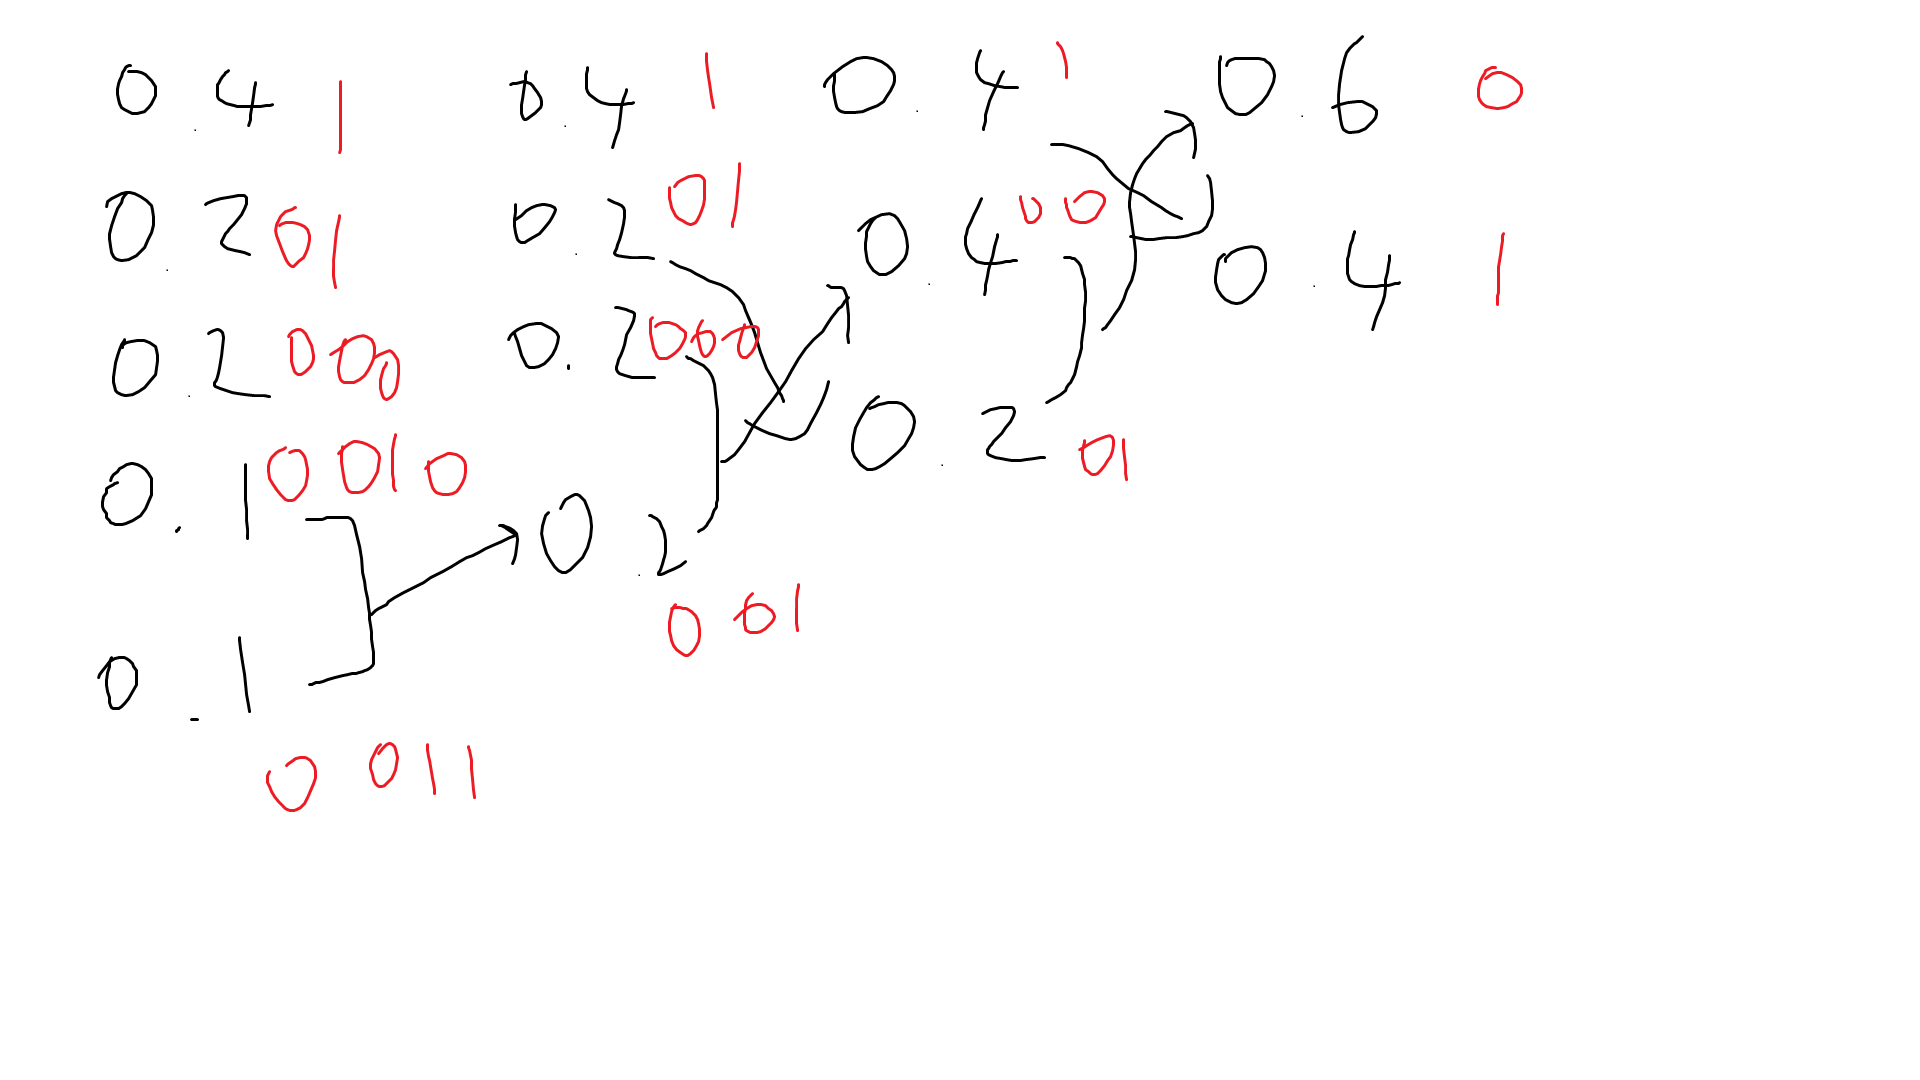
\includegraphics[scale=0.6]{image/CC_03.png}

So we get $\{1,01,000,0010,0011\}$ as the prefix-free code constructed. The expected word length is $2.$, which is better then the Shannon-Fano coding.
\end{eg}

\begin{thm} (1.5)\\
Huffman coding is optimal.
\end{thm}

\begin{lemma} (1.6) \\
Suppose $\mu_1,...,\mu_m \in \Sigma_1$ emitted with probabilities $p_1,...,p_m$. Let $f$ be an optimal prefix-free code with word lengths $s_1,...,s_m$. Then\\
(i) if $p_i > p_j$, then $s_i \leq s_j$;\\
(ii) there exists 2 codewords of maximal length which are equal up to the last digit.\\
\begin{proof}
(i) Otherwise, swap codewords $i$ and $j$ to reduce the expected word length.\\
(ii) If not, then either there is only one codeword of maximal length, or any two codewords of maximal length differ before the last digit. In either case, delete the last digit of each codeword of maximal length. This maintains the prefix free condition, contradicting with $f$ being optimal.
\end{proof}
\end{lemma}

\begin{proof} (of 1.5 ($a=2$))\\
We show, by induction on $m$, that any Huffman code of size $m$ is optimal.\\
$m=2$: codewords $0,1$ optimal;\\
$m>2$: source $X_m$ emits $\mu_1,...,\mu_m$ with probabilities $p_1 \geq p_2 \geq ... \geq p_m$. Source $X_{m-1}$ emits $\mu_1,...,\mu_{m-2},\nu$. with probabilities $p_1,...,p_{m-2},p_{m-1}+p_m$. We construct a Huffman coding $f_{m-1}$ for $X_{m-1}$ and extend to a Huffman coding for $X_m$. Then the expected codeword length satisfies $E(S_m) = E(S_{m-1}) + p_{m-1} + p_m$. Let $f'_m$ be an optimal code for $X_m$, wlog $f'_m$ prefix free. Lemma (1.6) shows that shuffling codewords we may assume that the last two codewords of $f'_m$ are of maximal length and differ only in the last digit, say $y_0$ and $y'$ (for some string $y$). We define a code $f'_{m-1}$ for $X_{m-1}$ with $f'_{m-1}(\mu_i) = f'_m (\mu_i)$ $\forall 1 \leq i \leq m-2$, $f'_{m-1} (\nu) =y$. Then $f'_{m-1}$ is a prefix free code and the expected word length satisfies $$E(S'_m) = E(S'_{m-1}) + p_{m-1}+p_m$$
By induction hypothesis, $f_{m-1}$ is optimal, so $E(S_{m-1}) \leq E(S'_{m-1}) \implies E(S_m) \leq E(S'_m)$, so $f_m$ is optimal.
\end{proof}

\begin{rem}
Not all optimal codes are Huffman. For example, if $p=0.3,0.3,0.2,0.2$, we could use code $00,10,01,11$ which is not Huffman.\\
Nevertheless, the previous result says if we have a prefix-free optimal code with word lengths $s_1,...,s_m$ associated with probabilities $p_1,...,p_m$, there exists a Huffman code with those word lengths.
\end{rem}

\begin{defi}
The \emph{joint entropy} of $X$ and $Y$ is
\begin{equation*}
\begin{aligned}
H(X,Y) = -\sum_{x \in \Sigma_1} \sum_{y \in \Sigma_2} P(X=x,Y=y) \log \P(X=x,Y=y)
\end{aligned}
\end{equation*}
\end{defi}

\begin{lemma}
$H(X,Y) \leq H(X) + H(Y)$, with equality iff $X$ and $Y$ independent.
\begin{proof}
Let $\Sigma_1 = \{x_1,...,x_m\}$, $\Sigma_2 = \{y_1,..,y_n\}$ $p_{ij} = \P(X=x_,Y=y_j)$, $p_i = \P(X=x_i), q_j = \P(Y=y_j)$. Apply Gibbs inequality with $p_{ij}$ and $p_i q_j$ we get
\begin{equation*}
\begin{aligned}
\sum p_{ij} \log (p_{ij}) & \leq -\sum p_{ij} \log (p_i q_j)\\
&= -\sum_i \sum_j p_{ij} \log p_i - \sum\sum p_{ij} \log q_j\\
&= -\sum p_i \log p_i - \sum q_j \log q_j
\end{aligned}
\end{equation*}
i.e. $H(x,y) \leq H(x) + H(Y)$. Equality holds iff $p_{ij} = p_i q_j$ $\forall i,j$ $\iff X,Y$ independent.
\end{proof}
\end{lemma}

Suppose we have a source $\Omega$ which produces a string $X_1,X_2,...$ of random variables with values in $\Sigma$. The probability mass function (pmf) of $X^{(n)} = (X_1,...,X_n)$ is given by $$p_n(x_1,...,x_n) = \P(X_1,...,X_n = x_1,...,x_n) \forall x_1,...,x_n \in \Sigma^n$$
Now $p_n: \Sigma^n \to \R$ by $X^{(n)}: \Omega \to \Sigma^n$. We can form $p(X^{(n)}: \Omega \xrightarrow{X^{(n)}} \Sigma^n \xrightarrow{p_n} \R$ by $w \to p_n(X^{(n)} = X^{(n)} (w))$ a random variable.

For example, let $\Sigma = \{A,B,C\}$. Then $X^{(2)} = AB (0.3), AC(0.1), BA(0.1), BA (0.2), CA(0.25), CB(0.05)$ So $p_2(AB)= 0.3$, etc.. And $p_2(X^{(2)})$ takes values $0.3$ with probability 0.3, 0.1 with probability 0.2, 0.2 with probaility 0.2, 0.25 with probability 0.25, 0.05 with probaility 0.05.

\begin{defi}
A sequence of random variables $X_1,...$ converges in probability to $c \in \R$, written $X_n \xrightarrow{p} c$ as $n \to \infty$, if $\forall \varepsilon >0$, $P(|x_n-c| \leq \varepsilon) \to 1$ as $n \to \infty$. So $X_n$ and $c$ can take very different values for large $n$ but only on a set with small probability.
\end{defi}

\begin{thm} (Weak law of large numbers)\\
Let $X_1,X_2,...$ be an i.i.d. sequence of random variables with finite expected value $\mu$, then $$\frac{1}{n} \sum_{i=1}^n X_i \xrightarrow{p} \mu$$
as $n \to \infty$.
\end{thm}

Application: Suppose $X_1,X_2,...$ is a Bernoulli source. Then $p(X_1),p(X_2),...$ are i.i.d. random variables, and $p(X_1,...,X_n) = p(X_1)...p(X_n)$. Take log of both sides we get 
$$-\frac{1}{n} \log p(X_1,...,X_n) = -\frac{1}{n} \sum_{i=1}^n \log p(X_i) \xrightarrow{p} \E(-\log p(X_1)) = H(X_1)$$
as $n \to \infty$.

\begin{defi}
A source $X_1,X_2,...$ satisfies the \emph{Asymptotic Equipartition Property} (AEP) if for some $H \geq 0$ we have
$$ -\frac{1}{n} \log p(X_1,...,X_n) \xrightarrow{p} H$$
as $n \to \infty$.
\end{defi}

Motivating example: suppose we have a coin with $p(H) = p$. If coin tossed $N$ times, expect approximately $pN$ heads and $(1-p)N$ tails. The probability of a particular sequence of $pN$ heads and $(1-p)N$ tails equals $p^{pN} (1-p)^{(1-p)N} = 2^{N(p\log p + (1-p) \log (1-p))} = 2^{-NH(A)}$, where $A$ is the result of independent coin toss. So, with high probability we will get a typical sequence, and its probability will be close to $2^{-NH(A)}$.

\begin{lemma} (1.8)\\
A source $X_1,X_2,...$ satisfies AEP iff it satisfies the following condition (*):\\
$\forall \varepsilon < 0, \exists n_0(\varepsilon) s.t. \forall n \geq n_0(\varepsilon) \exists$ a typical set $T_n \subset \Sigma^n$ s.t:\\
(i) $P((X_1,...,X_n) \in T_n) > 1-\varepsilon$;\\
(ii) $2^{-n(H+\varepsilon)} \leq p(x_1,...,x_n) \leq 2^{-n(H-\varepsilon)}$ for all $(x_1,...,x_n) \in T^n$.
\begin{proof} (sketch)\\
AEP $\implies$ (*):\\
Take $T_n = \{(x_1,...,x_n) \in \Sigma^n: |-\frac{1}{n} \log p(x_1,...,x_n) - H) < \varepsilon \} = \{(x_1,...,x_n) \in \Sigma^n : 2^{-n(H+\varepsilon)} \leq p(x_1,...,x_n) \leq 2^{-n(H-\varepsilon)}\}$.\\
(*) $\implies$ AEP:\\
$P(|-\frac{1}{n} p(X_1,...,X_n) - H| < \varepsilon) \geq P(T_n) \to 1$ as $n \to \infty$.
\end{proof}
\end{lemma}

\begin{defi}
A source $X_1,X_2,...$ is \emph{reliably encodable} at rate $r$ if there exists $A_n \subset \Sigma^n$ for each $n$ s.t.:\\
(i) $\frac{\log|A_n|}{n} \to r$ as $n \to \infty$;\\
(ii) $p((X_1,...,X_n) \in A_n) \to 1$ as $n \to \infty$.\\
So, in principle, you can encode at rate almost $r$ with negligible error for long enough strings.\\
So if $|\Sigma|=a$, you can reliably encode at rate $\log a$. However, you can often do better. For example, consider telegraph english with 26 letters and a space, we have $27 \approx 2^{4.755}$. So we can encode at a rate of $4.76$ bits/letter. But much lower rates suffice, there is a lot of redundancy in the english language. Hence the following definition:\\
\end{defi}

\begin{defi}
The \emph{information rate}, $H$, of a source, is the infimum of all rates at which it is reliably encodable.
\end{defi}

Roughly, $nH$, is the number of bits required to encode $(X_1,...,X_n)$.

\begin{thm} (1.9, Shannons' first encoding theorem)\\
If a source satisfies AEP with same constant $H$, then the source has information rate $H$.
\begin{proof}
Let $\varepsilon > 0$ and let $T_n \subset \Sigma^n$ be typical sets. Then for sufficiently large $n \geq n_0 (\varepsilon)$, $p(x_1,...,x_n) \geq 2^{-n(H+\varepsilon)}$ $\forall (x_1,...,x_n) \in T^n$.

So, $\P((X_1,...,X_n) \in T_n) \geq 2^{-n(H+\varepsilon)} |T_n| \implies |T_n| \leq 2^{n(H+\varepsilon)}$. So the source is reliably encodable at rate $H+\varepsilon$.\\
Conversely, if $H=0$ we are done. Otherwise, pick $0 < \varepsilon < \frac{H}{2}$. Suppose the source is reliably encodable at rate $H-2\varepsilon$, say with sets $A_n$. Then $p(x_1,...,x_n) \leq 2^{-n(H-\varepsilon)}$ $\forall (x_1,...,x_n) \in T_n$. This implies $P((x_1,...,x_n) \in A_n \cap T_n) \leq 2^{-n(H-\varepsilon)}|A_n|$, so $\frac{\log P(A_n \cap T_n}{n} \leq -(H-\varepsilon) + \frac{\log |A_n|}{n} \to -(H-\varepsilon) + (H-2\varepsilon) = -\varepsilon$ as $n \to \infty$. (??) So $\log p(A_n \cap T_n) \to -\infty$, i.e. $p(A_n \cap T_n) \to 0$. But $p(T_n) \to 1$ as $n \to \infty$ and $P(A_n) \to 1$ as $n \to \infty$, contradiction(??). So the source is not reliably encodable at rate $H-2\varepsilon$. So the information rate is $H$.
\end{proof}
\end{thm}

\begin{coro}
A Bernoulli source $X_1,X_2,...$ has information rate $H(X_1)$.
\end{coro}

\newpage

\section{Error control codes}

\begin{defi}
A $[n,m]$ binary code is a subset $C\subset \{0,1\}^n$  of size $|C| = m$. We say $C$ has length $n$. The elements of $C$ are called codewords.\\
Note: so this is a block codes.

We use a $[n,m]$ code to send one of $m$ possible messages through a BSC making use of the channel $n$ times. Suppose that we have a probability of $p$ that a digit get mistransmitted, i.e. $0$ becomes $1$ or the other way.
\end{defi}

\begin{defi}
The \emph{information rate} of $C$ is $\rho(C) = \frac{\log m}{n}$ (as usual, $\log$ is base 2).\\
Note since $C \subset \{0,1\}^n$, $\rho(C) \leq 1$, with equality iff $C = \{0,1\}^n$. A code with size $m=1$ has information rate $0$.\\
We aim to design codes with large information rate and small error rate. Apparently, these two are contradicting.
\end{defi}

The erro rate depends on the decoding rule. We consider 3 possible rules:\\
(i) The ideal observer: decoding rule decodes $x \in \{0,1\}^n$ as the codeword $c$ maximising $\P(c$ sent$| x$ received);\\
(ii) The maximum likelihood decoding rule decodes $x \in \{0,1\}^n$ as $c \in C$ maximising $\P(x$ received $| c$ sent);\\
(iii) The minimum distance decoding rule decodes $x\in\{0,1\}^n$ as $c \in C$ minimising the number of $\{1\leq i\leq n: x_i \neq c_i\}$, i.e. the manhattan distance.

\begin{rem}
Some convention should be agreed in the case of a 'tie', e.g. choose at random, or ask for message to be sent again.
\end{rem}

\begin{lemma}(2.1)\\
If all messages were equally likely, then (i) and (ii) agree.
\begin{proof}
By Bayes rule,
\begin{equation*}
\begin{aligned}
\P(c\ sent|x\ received) &= \frac{\P(c\ sent, x\ received)}{\P(x\ received)}\\
&= \frac{\P(c\ sent}{\P(x\ received)} \P(x\ received | c\ sent)
\end{aligned}
\end{equation*}
We suppose $P(c\ sent)$ is independent of $c$, so for fixed $x$ maximising $\P(c\ sent| x\ received)$ is the same as maximising $\P(x\ received | c\ sent)$.
\end{proof}
\end{lemma}

\begin{defi}
Let $x,y \in \{0,1\}^n$. Then \emph{Hamming distance} between $x$ and $y$ is $d(x,y) = |\{1\leq i \leq n: x_i \neq y_i\}|$.
\end{defi}

\begin{lemma} (2.2)\\
If $p < \frac{1}{2}$ then (ii) and (iii) agree.
\begin{proof}
Suppose $d(x,c) = r$. Then
\begin{equation*}
\begin{aligned}
\P(x\ received | c\ sent) = p^r (1-p)^{n-r} = (1-p)^n (\frac{p}{1-p})^r
\end{aligned}
\end{equation*}
since $p<1/2, \frac{p}{1-p} < 1$. So choosing $c$ to maximise the probability is the same as choosing $r$ to minimise the distance $d(x,c)$.
\end{proof}
\end{lemma}

Note that $p<\frac{1}{2}$ is really a reasonable assumption (else just revert everything we received).

\begin{eg}
Suppose codewords 000 and 111 are sent with probabilities $\alpha = \frac{9}{10}$ and $1-\alpha = \frac{1}{10}$ respecitvely. We use a BSC with $p=\frac{1}{4}$. If we receive 110 then we know by minimum distance to decode it as 111. By lemma (2.2), the maximum likelihood would give the same choice as well.\\
However, for ideal observer, we get $\P(000\ sent | 110\ received) = \frac{3}{4}$ (after some calculation). So ideal observer would decode as 000 (that's why it's ideal).
\end{eg}

\begin{rem}
Ideal observer rule is also known as minimum-error rule. However, it does rely on knowing the probability of the codewords sent.
\end{rem}

From now on we use minimum distance decoding.

\begin{defi}
(i) $C$ is $d$-error detecting if changing at mod $d$ letters of a codeword cannot give another codeword.\\
(ii) $C$ is $e$-error correcting if knowning that the string received has at most $e$ errors is sufficient to determine which codeword was sent.
\end{defi}

For example, the repetition code of length $n$, $C = \{000...0,111...1\}$ is $[n,2]$-code. It is $n-1$ error-detecting, and $\lfloor \frac{n-1}{2}\rfloor$-error correcting. But it's information rate is only $\frac{1}{n}$.

Another example: the simple parity check code of length $n$ (also known as paper tape code): we view $\{0,1\} = \Z/2\Z$, and $C = \{(x_1,...,x_n) \in \{0,1\}^n$, $\sum_{i=1}^n x_i = 0\}$.\\
This is a $[n,2^{n-1}]$ code. It is $1$-error detecting, but cannot correct any errors. It's information rate is $\frac{n-1}{n}$.

\begin{rem}
Suppose we change our code $C \subset \{0,1\}^n$ by using the same permutation to reorder each codeword. This gives a code with the same mathematical properties (e.g. information rate, error detection etc.). We say such codes are equivalent.\\
Suppose $d(x,c) = r$. Then
\begin{equation*}
\begin{aligned}
\P(x\ received | c\ sent) = p^r (1-p)^{n-r} = (1-p)^n (\frac{p}{1-p})^r
\end{aligned}
\end{equation*}
since $p<1/2, \frac{p}{1-p} < 1$. So choosing $c$ to maximise the probability is the same as choosing $r$ to minimise the distance $d(x,c)$.
\end{rem}

\begin{eg} (3, Hamming's original code, 1950)\\
Let $C \subseteq F_2^7$ be defined by\\
\begin{equation*}
\begin{aligned}
c_1+c_3+c_5+c_7=0\\
c_2+c_3+c_6+c_7=0\\
c_4+c_5+c_6+c_7=0\\
\end{aligned}
\end{equation*}
since we can choose $c_3,c_5,c_6,c_7$ freely, then $c_1,c_2,c_4$ is uniquely determined. We get $|C| = 2^4$, so $C$ is a $[7,16]$ code.\\
Information rate = $\frac{\log m}{n} = \frac{4}{7}$.\\
Suppose we receive $x \in F_2^7$. We form the syndrome $z_x = (z_1,z_2,z_4)$ where
\begin{equation*}
\begin{aligned}
z_1=x_1+x_3+x_5+x_7\\
z_2=x_2+x_3+x_6+x_7\\
z_4=x_4+x_5+x_6+x_7
\end{aligned}
\end{equation*}
if $x \in C$ then $z=(0,,0)$. If $d(x,c)=1$ for some $c \in C$, then the place where $x$ and $c$ differ is given by $z_1+2z_2+4z_4$ (not mod 2). So this is also $1$-error correcting.\\
Since if $x=c+e_1$ where $e_i = 0...010...0$ where $1$ is in the $i$th position, then the syndrome of $x$ is the syndrome of $e_1$, and for example syndrome of $e_3$ is $(1,1,0)$, the binary expansion of $3$. True for each $1 \leq i \leq 7$.
\end{eg}

Recall $d(x,y)$ is the number of differences between $x, y$.

\begin{lemma} (2.3)\\
The hamming distance is a metric on $F_2^n$.\\
Don't really want to copy the proof -- this is obvious.
\end{lemma}

Remark: we could also write $d(x,y) = \sum_{i=1}^n d_i (x_i,y_i)$ where $d_1$ is the discrete metric on $\{0,1\}$.

\begin{defi}
The minimum distance of a code $C$ is the smallest Hamming distance between distinct codewords.\\
An $[n,m]$-code with minimum distance $d$ is sometimes called an $[n,m,d]$-code.
\end{defi}

Note: $m \leq 2^n$, with equality if $C=F_2^n$, this is called the trivial code. Also $d \leq n$, with equality in the case of the repetition code.

\begin{lemma} (2.4)\\
Let $C$ be a code with minimum distance $d$.\\
(i) $C$ is $(d-1)$-error detecting, but cannot detect all sets of $d$ errors.\\
(ii) $C$ is $\lfloor \frac{d-1}{2}\rfloor$ error correcting, but cannot correct all sets of $\lfloor \frac{d-1}{2}\rfloor+1$ errors.
\begin{proof}
(i) If $x \in F_2^n$ and $c \in C$ with $1 \leq d(x,c) \leq d-1$, then $x \not\in C$, so errors detected. The second part is obvious.\\
(ii) Let $e = \lfloor \frac{d-1}{2}\rfloor$, so $e \leq \frac{d-1}{2} < e+1$, i.e .$2e < d \leq 2(e+1)$. Let $x \in F_2^n$. If $\exists c_1 \in C$ with $d(x,c_1) \leq e$, we want to show $d(x,c_2)>e$ $\forall c_2 \in C$, $c_2 \neq c_1$, which can be done by triangle inequality. So $C$ is $e$-error correcting. The second part is trivial as well.
\end{proof}
\end{lemma}

\begin{eg}
(1) The repetition code is a $[n,2,n]$-code, it is $n-1$ error detecting and $\lfloor \frac{n-1}{2}\rfloor$ error correcting.\\
(2) The simple parity check code is a $[n,2^{n-1},2]$-code. It is $1$-error detecting and $0$-error correcting.\\
(3) Hamming's original $[7,16]$-code is $1$-error correcting, i.e. $d \geq 3$. Since $0000000$ and $1110000$ are both in the code we get $d=3$, i.e. $[7,16,3]$-code.
\end{eg}

New codes from old:\\
Let $C$ be an $[n,m,d]$-code.\\
(i) The parity extension of $C$ is 
\begin{equation*}
\begin{aligned}
\bar{C} =\{(c,...,c_n,\sum c_i): (c_1,...,c_n) \in C\}
\end{aligned}
\end{equation*}
It is a $[n+1,m,d']$-code where $d \leq d' \leq d+1$.\\
(ii) Fix $1 \leq i \leq n$. Deleteing the $i^{th}$ letter from each codeword gives a punctured code. Assuming $d \geq 2$, $[n-1,m,d'']$ where $d-1 \leq d'' \leq d$.\\
(iii) Fix $1 \leq i \leq n$ and $a \in \{0,1\}$. The shortened code is $\{(c_1,...,c_{i-1},c_{i+1},...,c_n): (c_1,...,c_{i-1},a,c_{i+1},...,c_n) \in C\}$. It is a $[n-1,m',d']$-code where $d' \geq d$ and some choice of $a$ gives $m' \geq \frac{m}{2}$.

\subsection{Bound on codes}
\begin{defi}
Let $X \in F_2^n$ and $r \geq 0$. The (closed) Hamming ball with centre $x$ and radius $r$ is just what we think it will be (obvious). We denote it by $B(x,r)$.\\
Note that the volume $V(n,r) = |B(x,r)| =\ sum_{i=0}^r {n \choose i}$ is independent of $x$.
\end{defi}

\begin{lemma} (2.5, Hamming's bound)\\
If $C \subset \F_2^n$ is $e$-error correcting, then
\begin{equation*}
\begin{aligned}
|C| \leq \frac{2^n}{V(n,e)}
\end{aligned}
\end{equation*}
\begin{proof}
Since $C$ is $e$-error correcting, the Hamming Balls $B(c,e)$ are disjoint for $c \in C$. So done.
\end{proof}
\end{lemma}

\begin{defi}
A $[n,m]$-code which can correct $e$-errors is called \emph{perfect} if $m=\frac{2^n}{V(n,e)}$.
\end{defi}

Note that if $\frac{2^n}{V(n,e} \not\in \Z$ then no perfect $e$-erro correcting code of length $n$ can exist.

\begin{eg}
Hammings' original $[7,16,3]$-code can correct $1$ error. We can check that is is a perfect code.
\end{eg}

Note, however, that a perfect $e$-error correcting code will always incorrectly decode $e+1$ errors.

\begin{defi}
$A(n,d) = \max \{m: \exists\ a [n,m,d]-$code$\}$, i.e. size of largest code with parameters $n$ and $d$. For example, $A(n,1) = 2^n$, $A(n,n) = 2$.
\end{defi}

\begin{prop} (2.6)\\
\begin{equation*}
\begin{aligned}
\frac{2^n}{V(n,d-1)} \leq A(n,d) \leq \frac{2^n}{V(n,\lfloor \frac{d-1}{2} \rfloor}
\end{aligned}
\end{equation*}
The lower and upper bounds have alternative names: GSV-bounds and Hamming's bound.
\begin{proof}
We've already done the upper bound. For the lower bound, let $C$ be a code of length $n$ and minimum distance $d$ of largest possible size. Then $\not\exists x \in \F_2^n$ such that $d(x,c) \geq d$ $\forall c \in C$, otherwise we can place $C$ with $C \cup \{x\}$. So $\F_2^n \subseteq \cup_{c \in C} B(c,d-1)$, i.e. $|C| \geq \frac{2^n}{V(n,d-1)}$.
\end{proof}
\end{prop}

\begin{eg}
Consider $n=10,d=3$. Then $V(n,1) = 1+10=11$. $V(n,2) = 1+10+{10 \choose 2} = 56$. 2.6 gives $19 \leq A(10,3) \leq 93$. The exact value is 72, only known in 1999.
\end{eg}

There exist asymptotic versions of GSV and Hammings bound: Let $\alpha(\delta) = \limsup\frac{1}{n} \log A(n,\delta n)$, $0 \leq \delta \leq 1$.\\
Notation: $H(\delta) = -\delta\log\delta - (1-\delta) \log(1-\delta)$.\\
Asymptotic GSV boudn: $\alpha(\delta) \geq 1-H(\delta)$ for $0 < \delta < 1/2$;\\
Asymptotic Hamming: $\alpha(\delta) \leq 1-H(\delta/2)$.

We'll prove the asymptotic GSV bound.

\begin{prop} (2.7)\\
Let $0 < \delta < \frac{1}{2}$. Then\\
(i) $\log V(n,\lfloor n\delta\rfloor) \leq nH(\delta)$;\\
(ii) $\frac{\log A(n,\lfloor n\delta\rfloor}{n} \geq 1-H(\delta)$.
\begin{proof}
(i) $\implies$ (ii): GSV bound implies $A(n,\lfloor n\delta\rfloor) \geq \frac{2^n}{V(n,\lfloor n\delta \rfloor}$, so $\log A(n,\lfloor n\delta\rfloor) \geq n-\log V(n,\lfloor n\delta \rfloor) \geq n-nH(\delta)$ by (i). So $\frac{\log A(n,\lfloor n\delta\rfloor)}{n} \geq 1-H(\delta)$;\\
Proof of (i):
\begin{equation*}
\begin{aligned}
1 = (\delta + (1-\delta))^n &= \sum_{i=0}^n {n\choose i} \delta^i (1-\delta)^{n-i}\\
&\geq \sum_{i=0}^{\lfloor n\delta\rfloor} {n \choose i} \delta^i (1-\delta)^{n-i}\\
&= (1-\delta)^n \sum_{i=0}^{\lfloor n\delta\rfloor} {n \choose i} (\frac{\delta}{1-\delta})^i\\
&\geq (1-\delta)^n \sum_{i=0}^{\lfloor n\delta\rfloor} {n \choose i} (\frac{\delta}{1-\delta})^{n\delta}
\end{aligned}
\end{equation*}
Taking log, we get
\begin{equation*}
\begin{aligned}
0 \geq n(\delta\log\delta + (1-\delta) \log(1-\delta)) + \log V(n,\lfloor n\delta\rfloor)\\
\implies \log V(n,\lfloor n\delta \rfloor) \leq nH(\delta)
\end{aligned}
\end{equation*}
\end{proof}
\end{prop}

\subsection{Channel Capacity}
Let $|\Sigma| =q$. A code of length $n$ is a subset of $\Sigma^n$ (usually we take $q=2$).

A code is used to send messages through a discrete memoryless channel with $q$ imput letters. For each code a decoding rule is chosen.\\
We define $\hat{e}(C) = \max{c \in C} \P(error\ | c\ sent)$, the maximum error probability.

\begin{defi}
A channel can transmit reliably at rate $R$ if there exist a sequence of codes $C_1,C_2,...$ where $C_n$ is a code of length $n$ and size $\lfloor 2^{nR}\rfloor$ such that $\hat{e}(C_n) \to 0$.
\end{defi}

\begin{lemma} (2.8)\\
Let $\varepsilon>0$. A BSC with error probability $p$ is used to send $n$ digits. Then the probability of the BSC making at least $n(p+\varepsilon)$ errors $\to 0$ as $n \to \infty$.
\begin{proof}
Let $\mu_i = 1$ if digit mistransmitted, $0$ otherwise. Then $\mu_1,...$ are iid rvs. Also $P(\mu_i=1) = p$, so $E(\mu_i) = p$. So the require probability is $P(\sum_{i=1}^n \mu_i \geq n(p+\varepsilon)) \leq \P(|\frac{1}{n} \sum \mu_i-p| \geq \varepsilon) \to 0$ as $n \to \infty$ by WLLN.
\end{proof}
\end{lemma}

Remark: $\sum_{i=1}^n \mu_i$ is a binomial rv with parameters $n$ and $p$.

\begin{prop} (2.9)\\
The capacity of a BSC with error probability $p<1/4$ is not zero.
\begin{proof}
Choose $\delta$ with $2p < \delta < 1/2$. We prove reliably encoding at rate $R=1-H(\delta)>0$. Let $C_n$ be the largest code of length $n$ and minimum distance $\lfloor n\delta\rfloor$. So $|C_n| = A(n,\lfloor n\delta\rfloor) \geq 2^{n(1-H(\delta))} = 2^{nR}$ by (2.7). Replacing $C_n$ by a subcode gives $|C_n| = \lfloor 2^{nR}\rfloor$ and still minimum distance $\geq \lfloor n\delta\rfloor$. Using minimum distance decoding,
\begin{equation*}
\begin{aligned}
\hat{e}(C_n) &\leq P(BSC \text{ makes} \geq \lfloor \frac{\lfloor n\delta-1}{2}\rfloor+1 \text{ errors} )\\
&\leq P(BSC \text{ makes} \geq \frac{n\delta-1}{2} \text{ errors})
\end{aligned}
\end{equation*}
Pick $\varepsilon > 0$ s.t. $p+\varepsilon < \frac{\delta}{2}$. Then $\frac{n\delta-1}{2} = n(\frac{\delta}{2}-\frac{1}{2n}) > n(p+\varepsilon)$ for $n$ sufficiently large. So $\hat{e}(C_n) \leq P(BSC \text{ makes} \geq n(p+\varepsilon) \text{ errors}) \to 0$ as $n \to \infty$ by (2.8).
\end{proof}
\end{prop}

\subsection{Conditional Entropy}

Let $X$ and $Y$ be random variables taking values in $\Sigma_1$ and $\Sigma_2$. We define
\begin{equation*}
\begin{aligned}
H(X | Y=y) = -\sum_{x \in \Sigma_1} P(X=x|Y=y) \log P(X=x|Y=y),\\
H(X|y) = \sum_{y \in \Sigma_2} P(Y=y)H(x|Y=y)
\end{aligned}
\end{equation*}

\begin{lemma} (2.10)\\
$H(X,Y) = H(X|Y) + H(Y)$.
\begin{proof}
\begin{equation*}
\begin{aligned}
H(X|Y) &= -\sum_{y \in \Sigma_2} \sum_{x \in \Sigma_1} P(X=x|Y=y) P(Y=y) \log P(X=x|Y=y)\\
&= -\sum_{y \in \Sigma_2} \sum_{x \in \Sigma_1} P(X=x,Y=y) \log \frac{P(X=x,Y=y)}{P(Y=y)}\\
&= -\sum_{y \in \Sigma_2} \sum_{x \in \Sigma_1} P(X=x,Y=y) \log P(X=x,Y=y) + \sum_{y \in \Sigma_2} (\sum_{x \in \Sigma_1} P(X=x,Y=y) ) \log P(Y=y)\\
&= H(X,y) - H(y)
\end{aligned}
\end{equation*}
\end{proof}
\end{lemma}

Example: A fair six sided dice is thrown. $X$ is the value on the dice, $y=X mod 2$. So $H(X,Y) = H(X) =\log 6$, $H(y) = \log 2 = 1$, $H(X|Y) = H(X,Y)-H(Y)= \log 3$, and $H(Y|X) = 0$.


\begin{coro}
$H(X|Y) \leq H(X)$ with equality iff $X$ and $Y$ are independent.
\begin{proof}
Since $H(X|Y) = H(X,Y) - H(Y)$, this is equivalent to $"H(X,Y) \leq H(X)+H(Y)$ with equality iff $X$ and $Y$ independent, which is true by (1.7).
\end{proof}
\end{coro}

In the definition of conditional entropy, we can replace random variables $X$ and $Y$ with random vectors $X=(X_1,...,X_r$ and $Y=(Y_1,...,Y_s)$. This defines $H(X_1,...,X_r| Y_1,...,Y_s)$.

\begin{lemma} (2.11)\\
$H(X|Y) \leq H(X|Y,Z) + H(Z)$.
\begin{proof}
We expand $H(X,Y,Z)$ using (2.10) in two different ways:
$H(X,Y,Z) = H(Z|X,Y)+H(X|Y)+H(Y)$ and $H(X,Y,Z)=H(X|Y,Z)+H(Z|Y)+H(Y)$. Since $H(Z|X,Y)\geq 0$, we get $H(X|Y)\leq H(X|Y,Z)+H(Z|Y)\leq H(X|Y,Z)+H(Z)$ by corollary.
\end{proof}
\end{lemma}

\begin{lemma} (2.12, Fano's inequality)\\
Let $X,Y$ be random variables taking values in $\Sigma_1$ with $\Sigma_1 | = m$. Let $p = P(x \neq y)$. Then $H(X|Y) \leq H(p) + p\log (m-1)$.
\begin{proof}
Let $Z=1$ if $X\neq Y$, and 0 oterwise. Then $P(Z=1) = p$. So by (2.11),
\begin{equation*}
\begin{aligned}
H(X|Y) \leq H(X|Y,Z)+\underbrace{H(Z)}_{=H(p)} \ (*)
\end{aligned}
\end{equation*}
Now $H(X|Y=y,Z=0) = 0$ (must have $X=y$), $H(X|Y=y,Z=1) \leq \log (m-1)$ since $m-1$ choices for $X$ remain. So, $H(X|Y,Z) = \sum_{y,z} P(Y=y,Z=z) H(X|Y=y,Z=z) \leq \sum_y P(Y=y,Z=1) \log (m-1)$, where the sum is just $P(Z=1)=p$ and by (*) we get the result.
\end{proof}
\end{lemma}

\begin{defi}
Let $X,Y$ be random variables. The mutual information is 
\begin{equation*}
\begin{aligned}
I(X,Y) = H(X)-H(X|Y)
\end{aligned}
\end{equation*}
i.e. the amount of information about $X$ conveyed by $Y$.
\end{defi}

By (1.7) and (2.10), we have $I(X,Y) = H(X)+H(Y)-H(X,Y) \geq 0$ is symmetric in $X$ and $Y$. We get equality iff $X$ and $Y$ are independent.

consider a DMC. Let $X$ takes values in $\Sigma_1$, where $|\Sigma_1 = m$ with probabilities $p_1,...,p_m$. Let $Y$ be the random variable output when channel is given input $X$. 

\begin{defi}
The \emph{information channel capcity} is $\max_X I(x;y)$.
\end{defi}

\begin{rem}
The $\max$ is over all choices of $p_1,...,p_m$; $\max$ is always attained since $I$ is continuous on a compact set.\\
The information capacity only depnds on the channel matrix.
\end{rem}

\begin{thm} (2.13, Shannon's Second Coding Theorem)\\
Operational capacity = information capacity. (LHS?)

We'll show $\leq$ in general, and $\geq$ for a BSC.
\end{thm}

We now compute the capacity of certain channels using Shannon's second coding theorem (error probability $p$):\\
Input $X$, $P(X=0) = 1-\alpha$, $P(X=1) = \alpha$, output $Y$, $P(Y=0) = (1-\alpha)(1-p) +\alpha p$, $P(Y=1) = \alpha(1-p) + (1-\alpha)p$.

Capacity is 
\begin{equation*}
\begin{aligned}
C &= \max_\alpha I(X,Y)\\
&= \max_\alpha(H(Y) - H(Y|X))\\
&= \max_\alpha(H(\alpha(1-\beta)+(1-\alpha)\beta) - H(p))\\
&= 1-H(p) \text{ max attained when } \alpha=1/2\\
&= 1+p\log p + (1-p) \log (1-p)
\end{aligned}
\end{equation*}
Here we denote $H(p) = H(p,1-p)$.

Capacity of Binary Erasive Channel (erasive probability $p$):\\
In this model we have each bit having a probability of $p$ being erased to become a $*$.\\
Input $X$, $P(X=0) = 1-\alpha$, $P(X=1) = \alpha$; output $Y$, $P(Y=0) = (1-\alpha)(1-p)$, $P(Y=1) = \alpha(1-p), P(Y=*) = p$. Now $H(X|Y=0) = 0$, $H(X|Y=1) = 0$. The only interesting case is 
\begin{equation*}
\begin{aligned}
H(X|Y=*) &= -\sum_x P(X=x|Y=*) \log P(X=x|Y=*)\\
&= H(\alpha)
\end{aligned}
\end{equation*}
where we work out
\begin{equation*}
\begin{aligned}
P(X=0|Y=* = 1-\alpha, P(X=1|Y=*) = \alpha
\end{aligned}
\end{equation*}
Capacity is 
\begin{equation*}
\begin{aligned}
C&=\max_\alpha I(X,Y)\\
&=\max_\alpha (H(X)-H(X|Y))\\
&= \max_\alpha (H(\alpha) - pH(\alpha))\\
&= (1-p) \max_\alpha H(\alpha)\\
&= 1-p
\end{aligned}
\end{equation*}
attained when $\alpha = 1/2$.

We model using a channel $n$ times as the $n^{th}$ extension, i.e. we replace input and output alphabets $\Sigma_1$ and $\Sigma_2$ by $\Sigma_1^n$ and $\Sigma_2^n$. Channel probabilities: $P(y_1...y_n\ received | x_1...x_n\ sent =\ prod_{i=1}^n P(y_i\ received| x_i\ send)$.

\begin{lemma} (2.14)\\
The $n^{th}$ extension of a DMC with information capacity $C$ has information capacity $nC$.
\begin{proof}
We take r.v. input $X_1,...,X_n = X$ producing r.v. output $Y_1,...,Y_n = Y$. Now
\begin{equation*}
\begin{aligned}
H(Y|X = \sum_x P(X=x) H(Y|X=x)
\end{aligned}
\end{equation*}
Since channel is memoryless,
\begin{equation*}
\begin{aligned}
H(Y|X=x) = \sum_i H(Y_i|X=x) = \sum_i H(Y_i|X_i=x_i)
\end{aligned}
\end{equation*}
So
\begin{equation*}
\begin{aligned}
H(Y|X) &= \sum_x P(X=x) \sum_i H(Y_i|X_i = x_i)\\
&= \sum_i \sum_n H(Y_i|X_i = n) P(X_i = n)\\
&= \sum_i H(X_i | Y_i)
\end{aligned}
\end{equation*}
Now $H(Y) \leq H(Y_1)+...+H(Y_n)$ by (1.7). So $I(X,Y) = H(Y)-H(Y|X) \leq \sum_i (H(Y_i)-H(Y_i|X_i)) = \sum_{i=1}^n I)X_i,Y_i) \leq nC$ by definition of info capacity.

For equality, we need $Y_1,...,Y_n$ to be independent. This can be achieved by taking $X_1,...,X_n$ independent and choosing the distribution s.t. $I(X_i,Y_i) = C$.
\end{proof}
\end{lemma}

\begin{prop} (2.15)\\
For a DMC, operational capacity $\leq$ information capacity.
\begin{proof}
Let $C$ be the information capacity. Suppose we can transmit reliably at rate $R>C$, i.e. there is a sequence of codes $(C_n)_{n \geq 1}$ with $C_n$ of length $n$ and size $\lfloor 2^{nR} \rfloor$ such that $\hat{e}(C_n) \to 0$ as $n \to \infty$. Then $\hat{e}(C_n) = \max_{c \in C_n} P(error | c\ sent)$, $e(C_n) = \frac{1}{|C_n|} \sum_{c \in C_n} P(error|\ sent)$. Clearly $e(C_n) \leq \hat{e}(C_n)$, so $e(C_n) \to 0$ as $n \to \infty$. Take r.v. input $X$, equidistributed over $C_n$. Let $Y$ be the r.v. output when $X$ is transmitted and decoded. So $e(C_n) = P(x \neq y) = p$ say.\\
Now $H(X) = \log (|C_n|) \geq nR-1$ for $n$ sufficiently large, $H(X|Y) \leq H(p) + p\log (|C_n|-1) \leq 1+pnR$ (Fano's inequality), $I(X,Y) = H(X) - H(X|Y)$, $nC \geq nR-1 - (1+pnR)$ (2.14), so $pnR \geq n(R-C)-2$. So we get $p \geq \frac{n(R-C)-2)}{nR} \not\to 0$ as $n \to \infty$.\\
Thus our sequence of codes cannot exist.
\end{proof}
\end{prop}

\begin{prop} (2.16)\\
Consider a BSC, erro probability $p$. Let $R < 1-H(p)$. Then ther exists a sequence of codes $(C_n)_{n \geq 1}$ of length $n$ and size $\lfloor 2^{nR}\rfloor$ such that $e(C_n) \to 0$ as $n \to \infty$.
\begin{proof}
The idea is to construct codes by picking codewords at random. WLOG let $p<1/2$, so $\exists \varepsilon>0$ s.t. $R<1-H(p+\varepsilon)$. We use minimum distance decoding (in case of tie, make arbitrary choice).\\
Let $m = \lfloor 2^{nR}\rfloor$. We pick a $[n,m]-$code $C$ at random (i.e. each with probability $\frac{1}{{2^n \choose m}}$, say $C=\{c_1,...,c_m\}$. Choose $1 \leq i \leq m$ at random (i.e. each with probability $1/m$). We send $c_1$ through the channel and get output $Y$.\\
Then $P(Y$ is not decoded as $c)$ is the average value of $e(C)$ as $C$ runs over all $[n,m]-$codes. We can pick $C_n$ a $[n,m]-$code with $e(C_n)$ at most this average. So it will suffice to show that
\begin{equation*}
\begin{aligned}
P(Y \text{ is not decoded as } c_i) \to 0 \text{ as }n \to \infty
\end{aligned}
\end{equation*}
Let $r = \lfloor n(p+\varepsilon)\rfloor$. Then the above probability $\leq$ $P(C_i \not\in B(Y,r)) + P(B(Y,r) \cap C \supsetneq \{c_i\})$, i.e. either $c_i$ is not in the ball, or it is in the ball but is not the only one. We consider the two probabilities separately:\\
(i) $P(d(c_i,y) > r) = P($ BSC makes $>r$ errors$) = P($ BSC makes $>n(p+\varepsilon)$ errors$) \to 0$ as $n \to \infty$ by WLLN. \\
(ii) if $j \neq i$, $P(c_j \in B(Y,r) | c_i \in B(Y,r)) = \frac{V(n,r) - 1}{2^n-1} \leq \frac{V(n,r)}{2^n}$. So,
\begin{equation*}
\begin{aligned}
P(B(Y,r) \cap C \supsetneq \{c_i\}) &\leq (m-1) \frac{V(n,r)}{2^n}\\
&\leq 2^{nR} 2^{nH(p+\varepsilon)} 2^{-n}\\
&= 2^{n(R-(1-H(p+\varepsilon)))} \to 0
\end{aligned}
\end{equation*}
as $n \to \infty$, since $R<1-H(p+\varepsilon)$.
\end{proof}
\end{prop}

\begin{prop} (2.17)\\
Consider a BSC with error probaiblity $p$. Let $R<1-H(p)$. Then there exists a sequence of codes $(C_n)_{n \geq 1}$ with $C_n$ of length $n$, size $\lfloor 2^{nR}\rfloor$ and $\hat{e}(C_n) \to 0$ as $n \to \infty$.
\begin{proof}
Pick $R'$ s.t. $R < R' < 1-H(p)$. By (2.16), we construct a sequence of codes $(C'_n)_{n \geq 1}$ with $C'_n$ of length $n$, size $\lfloor 2^{nR} \rfloor$ and $e(C'_n) \to 0$ as $n \to \infty$.\\
Throwing at the worst half of the codewords in $C'_n$, gives a code $C_n$ with $\hat{e}(C_n \leq 2e(C'_n)$. So $\hat{e}(C_n) \to 0$ as $n \to \infty$.\\
Note $C_n$ has length $n$ and size $\lfloor 2^{nR-1} \rfloor$, but $2^{nR-1} = 2^{n(R'-[frac{1}{n}} \geq 2^{nR}$ for $n$ sufficiently large.\\
We can replace $C_n$ by a subcode of size $\lfloor 2^{n+R}\rfloor$ and still get $\hat{e}(C_n) \to 0$ as $n \to \infty$.
\end{proof}
\end{prop}

Conclusion: a BSC with error probaility $p$ has operational capacity $1-H(p)$.

Remark: (i) How does it work? say capcity is 0.8, and we have a message a string of $0's$ and $1's$. Let $R=0.7s < 0.8$, Then $\exists$ a set of $2^{0.75n}$ codewords of length $n$ that have error probability below some prescribed threshold, hence to encode message:\\
(a) break message into block's of size $3\lceil[\frac{n}{4}\rceil = m$ sufficiently large;\\
(b) encode these $m$-blocks into $C_n$ using codewords of length $\frac{4}{3} m$ each $m$ block;\\
(c) transmit new message through channel.\\

The theorem shows good codes exists. But the proof does not construct them for us.

\subsection{Linear codes}
In practice, we consider codes with extra strucutre to allow efficient decoding.

\begin{defi}
A code $C \subset F_2^n$ is linear if:\\
(i) $0 \in C$;\\
(ii) If $x,y \in C$, then $x+y \in C$.
\end{defi}

Recall: $F_2 =\{0,1\}$ the field with $2$ elements, addition and multiplication are mod 2. Equivalently, $C \subset F_2^n$ is linear if its an $F_2$ vector space.

\begin{defi}
The \emph{rank} of a linear code $C$ is its dimension as an $F_2$ vector space.
\end{defi}

A code $C$ of length $n$ and rank $k$ is called an $(n,k)$-code.

We say $C$ has a basi s$v_1,...,v_k$. Then $C = \{\sum \lambda_i v_i: \lambda_i \in F_2\}$ so $|C|=2^k$, i.e. a $(n,k)$-code is a $[n,2^k]$ code. The information rate is $\frac{k}{n}$.

For $x,y \in F_2^n$, we defined $x \cdot y = \sum_{i=1}^n x_i y_i \in F_2$ i.e. the inner product. Note this is commutative, and distributive. But note $x \cdot x = 0 \not\implies x = 0$.

\begin{lemma} (2.18)\\
Let $P \subset F_2^n$ be a subset. Then $C = \{x \in F_2^n : p \cdot x = 0 \forall p \in P\}$ is a linear code.
\begin{proof}
(i) $0 \in C$ since $p \cdot 0 = 0$ $\forall p \in P$.\\
(ii) If $x,y \in C$, then $p \cdot (x+y) = p\cdot x + p \cdot y = 0$, so $x+y \in C$.
\end{proof}
\end{lemma}

$P$ is called a set of \emph{parity checks} and $C$ is a \emph{parity check code}.

\begin{defi}
Let $C \subset F_2^n$ be a linear code. The \emph{dual code}
\begin{equation*}
\begin{aligned}
C^\perp = \{x \in F_2^n : x \cdot y = 0 \forall y \in C\}
\end{aligned}
\end{equation*}
by (2.18), $C^\perp$ is a code.
\end{defi}

\begin{lemma} (2.19)\\
$\dim C + \dim C^\perp = n$.\\
Note that these two sets might have non-empty intersection.
\begin{proof}
$V=F_2^n$, $V^* = $ linear maps from $V \to F_2$. Consider $\varphi: V \to V^*$ by $x \to \theta_x$ where $\theta_x: y \to x \cdot y$. Then $\varphi$ is a linear map. Suppose $x \in \ker \varphi$, then $x \cdot y = 0$ $\forall y \in V$. Taking $y = e_i = (0...010..0)$ ($i$th place is 1) gives $x_i = 0$. So $\ker \varphi = \{0\}$. Since $\dim V = \dim V^*$ (LA), it follows that $\varphi$ is an isomorphism. Thus $\phi(C^\perp) = \{\theta \in V^*: \theta(x) = 0 \forall x \in C\}$, i.e. the annihilator of $C$, denoted by $C^\circ$. By Linear algebra we know $\dim C + \dim C^\circ = \dim V = n$.
\end{proof}
\end{lemma}

\begin{coro}
$(C^\perp)^\perp = C$ for any linear code $C$. In particular, any linear code is a partiy check code.
\begin{proof}
Let $x \in C$. Then $x \cdot y = 0 \forall y \in C^\perp \implies x \in (C^\perp)^\perp$, i.e. $C \subseteq (C^\perp)^\perp$. By (2.19) twice, $\dim(C^\perp)^\perp = \dim C$, so $C = (C^\perp)^\perp$.
\end{proof}
\end{coro}

\begin{defi}
Let $C$ be a $(n,k)$ linear code.\\
(i) A generator matrix for $C$ is a $k \times n$ matrix whose rows are a basi for $C$.\\
(ii) A parity check matrix for $C$ is a generator matrix for $C^\perp$. It is a $(n-k)\times n$ matrix.
\end{defi}

\begin{defi} (2.20)\\
Every $(n,k)$ linear code is equivalent to a linear code with generator matrix $(I_k|B)$.
\begin{proof}
We can perform row operations: swap 2 rows or add one row to another (multiplying by scalars is not useful here).\\
By Gaussian elimination, we get $G$, the generator matrix in row echelon form, i.e. $\exists l(1) < l(2) < ... < l(n)$ s.t. $G_{ij} = 0$ if $j<l_i$ and $1$ if $j=l(i)$. Permuting the columns of $G$ gives an equivalent code, i.e. $l(i) = 1$ for $1 \leq i \leq k$. More row operations put $G$ in the form $(I_k|B)$ with $B$ a $k \times (n-k)$ matrix.
\end{proof}
\end{defi}

\begin{rem}
A message $y\in F_2^k$ (a row vector) is sent as $yG$. If $G = (I_k |B)$ then $yG = (y|yB)$, where we can see $y$ as message and $yB$ as check digits.
\end{rem}

\begin{lemma} (2.21)\\
A $(n,k)$ linear code with generator matrix $G = (I_k|B)$ has parity check matrix $H=(-B^T | I_{n-k})$.
\begin{proof}
Since $GH^T = -B+B =0$, we know rows of $H$ generate a subcode $C^\perp$. But $\dim (C^\perp) = n-k = r(H)$ as $H$ has $I_{n-k}$ as submatrix. So the rows of $H$ are a basis for $C^\perp$ as required.
\end{proof}
\end{lemma}

Hamming weight: the weight of $x \in F_2^n$ is $N(x) = d(x,0)$.

\begin{lemma} (2.22)\\
The minimum distance of a linear code $C$ is the minimum weight of a non-zero codeword.
\begin{proof}
Let $x,y \in C$. Then $x+y \in C$, and $d(x,y) = d(x-y,0) = d(x+y,0) = w(x+y)$. Note $x,y$ distinct means $x+y \neq 0$, so $d(C) = \min_{x,y \in C distinct} d(x,y) = \min_{z \in C,z \neq 0} w(z)$.
\end{proof}
\end{lemma}

\begin{defi}
The weight $w(C)$ of a linear code $C$ is the minimum weight of a non-zero codeword.

By (2.22), this is the same as minimum distance.
\end{defi}

\subsection{Syndrome Decoding}
Let $C$ be a $(n,\hat{k})$-linear code with parity check matrix $H$. Then $C =\{x \in F_2^n: Hx = 0\}$ where $x$ is a column vector.

Suppose we receive $y=c+e$ where $c \in C$ is a codeword and $e \in F_2^n$ is an error. We compute the \emph{syndrome} $Hy$. Suppose we know $C$ is $k$-error correcting. Then we tabulate the syndromes $He$ for all $e \in F_2^n$ with $w(e) \leq k$. If we receive $y$ we search for $Hy$ in our list. If successful, we get $Hy = He$ for some $e \in F_2^n$ with $w(e) \leq k$. We decode $y$ as $c = y-e$. Then $c \in C$ as $Hc = Hy-He = 0$ and $d(y,c) = w(e) \leq k$.

Recall Hamming's original code: $c_1+c_3+c_5+c_7 = 0$, $c_2+c_3+c_6+c_7 = 0$, $c_4+c_5+c_6+c_7 = 0$. So $c^\perp = \bra (1010101),(0110011),(0001111)\ket$. So 
\begin{equation*}
\begin{aligned}
H=\begin{pmatrix}
1010101\\
0110011\\
0001111
\end{pmatrix}
\end{aligned}
\end{equation*}
and $Hy = z = (z_1 z_2 z_4)$.

In general we have Hamming codes: let $d \geq 1, n = 2^d-1$. Let $H$ be the $d \times n$ matrix whose columns are the non-zero elmeents of $F_2^d$. The hamming $(n-n-d)$ linear code is the linear code with parity check matrix $H$ (original is $d=3$).

\begin{lemma} (2.23)\\
Let $C$ be a linear code with parity check matrix $H$. Then $w(C) = d$ iff\\
(i) any $(d-1)$ columns of $H$ are linearly independent;\\
(ii) some $d$ columns of $H$ are linearly dependent.
\begin{proof}
Suppose $C$ has length $n$. Then $C = \{x \in F_2^n: Hx = 0\}$. If $H$ has columnts $v_1,...,v_n$. Then
\begin{equation*}
\begin{aligned}
(x_1,,...,x_n) \in C \iff \sum_{i=1}^n x_i v_i = 0
\end{aligned}
\end{equation*}
i.e. code words are dependence relations between columns.
\end{proof}
\end{lemma}

\begin{lemma} (2.24)\\
The Hamming $(n,n-d)$ linear code has minimum distance $d(C) = 3$, and is a perfect $1$-error correcting code.
\begin{proof}
Any two columns of $H$ are linearly independent (where $H$ is the parity check matrix of $C$, but there exists $3$ that are linearly dependent. Hence $d(C) = 3$ by (2.23). And (2.4) says $C$ is a 1-error correcting code. To be perfect: $|C| = \frac{2^n}{V(n,e)}$, here $n = 2^d - 1$, $e=1$, so $\frac{2^n}{V(n,e)} = \frac{2^n}{1+2^d-1} = 2^{n-d} = |C|$.
\end{proof}
\end{lemma}

New codes from old:

The following construction is specific to linear code.

\begin{defi}
Let $C_1$, $C_2$ linear codes of length $n$ with $C_2 \subseteq C_1$, i.e. $C_2$ is a subcode of $C_1$. The \emph{bar product} is 
\begin{equation*}
\begin{aligned}
C_1 | C_2 = \{(x|x+y): x \in C_1, y \in C_2\}
\end{aligned}
\end{equation*}
is a linear code of length $2n$.

\begin{lemma} (2.25)\\
Let $C_1,C_2$ be as above.\\
(i) $rk (C_1|C_2) = rank(C_1)+rk(C_2)$;\\
(ii) $w(C_1|C_2) = \min \{2w(C_1),w(C)2)\}$.
\begin{proof}
(i) Let $x_1,...,x_k$ be basis for $C_1$. Let $y_1,...,y_l$ be basis for $C_2$. Then $\{(x_i|x_i) : 1 \leq i \leq k\} \cup \{(0 | y_i): 1 \leq j \leq l\}$ is a basis for $C_1 | C_2$, hence $rank(C_1|C_2) = rank(C_1)+rank(C_2)$.\\
(ii) Let $x \in C_1$, $y \in C_2$ not both zero. If $y \neq 0$: $w(x|x+y) = w(x)+w(x+y) \geq w(y \geq w(C_2)$. If $y=0$ (so $x \neq 0$), $w(x|x) = 2w(x) \geq 2w(C_1)$. So $w(C_1|C_2) \geq \min \{2w(C_1),w(C_2)\}$. But there exists $0 \neq x \in C_1$ s.t. $w(x) = w(C_1)$, so $w(x) = 2w(x) = 2w(C_1)$; So $w(0|y) = w(y) = w(C_2)$. So $w(C_1|C_2) = \min\{2w(C_1), w(C_2)\}$.
\end{proof}
\end{lemma}
\end{defi}

\subsection{Reed-Muller Codes}
Let $X = F_2^d = \{p_1,...,p_n\}$ where $n=2^d$ (chosen an ordering). For $A \subseteq X$, we get a vector $1_A \in F_2^n$ by the rule $(1_A)_i = 1 \iff p_i \in A$, i.e. $1_A$ is the indicator function of $A$.

For $x,y \in F_2^n$, we have $x+y = (x_1+y_1,...,x_n+y_n)$, $x \wedge y = (x_1y_1,...,x_ny_n)$, then $(F_2^n,+,\wedge)$ is aring.

For $A,B \subseteq X$ we have $1_A+1_B = 1_{A \triangle B}$ where $\triangle$ is the symmetric difference: $A \triangle B = A \cap B \setminus A \cup B$, and $1_A \cup 1_B = 1_{A \cup B}$.\\
$w(1_A) = |A|$.

Let $v_0 = 1_x = (1,...,1)$ (multiplicative identity).

For $1 \leq i \leq d$, let $v_i = 1_{H_i}$ where $H_i = \{p \in X: p_i = 0\}$.

\begin{defi}
Let $0 \leq r \leq d$. The Reed-Muller code $RM(d,r)$ of order $r$ and length $2^d$ is the vector subspace of $F_2^n$ spanned by $v_0$ and wedge products of at most $r$ of the $v_i$.\\
Convention: the wedge product with zero terms is $v_0$.
\end{defi}

For example, consider $d=3$. We have $v_0 = 11111111,v_1 = 11110000,v_2=11001100,v_3 = 10101010$, and we can calculate their wedge products correspondingly. We have $RM(3,0)$ is spanned by $v_0$. It is the repetition code of length 8; $RM(3,1)$ is spanned by $v_0,v_1,v_2,v_3$. Deleteing the 1st component gives Hamming's $(7,4)$-code, i.e. the last 7 digits of $v_i$ are generator matrix for Hamming's $(7,4)-$code. Note also that all $v_i$ have even weight. So $RM(3,1)$ is equivalent to the partiy check extension of Hamming's $(7,4)-$code.\\

$RM(3,2)$ is spanned by $v_0,v_1,v_2,v_3,v_1 \wedge v_2,v_2 \wedge v_3,v_3 \wedge v_1$. These are linearly independent (see next theorem), so $RM(3,2)$ is a $(8,)7$-code. Each codeword has even weight, so $RM(3,2)$ is the simple parity check code of length $8$.

Lastly, $RM(3,3)$ is the trivial code.

\begin{thm} (2.26)\\
(i) The vectors $v_{i_1} \wedge ... \wedge v_{i_s}$ for $1 \leq i_1 < ... < i_s < d$ and $0 \leq s \leq d$ are a basis for $F_2^n$.\\
(ii) $RM(d,r)$ has rank $\sum_{s=0}^r {d \choose r}$.\\
(iii) $RM(d,r) = RM(d-1,r) | RM(d-1,r-1)$.\\
(iv) $RM(d,r)$ has weight $2^{d-r}$.
\begin{proof}
(i) We have a set of $\sum_{s=0}^d = 2^d = n$ vectors, so it suffices to show they span $F_2^n$, equivalently $R(d,d) = F_2^n$. Let $p \in X$. Let $y_i = v_i$, if $p_i=0$, or $v_0+v_i$ if $p_i = 1$. Then $1_{\{p\}} = y_1 \wedge y_2 \wedge ... \wedge y_d$. Expanding using distributive law gives that $1_{\{p\}} \in RM(d,d)$. But these indicator functions form a spanning set.\\
(ii) By definition, $RM(d,r)$ is spanned by the vectors $v_{i_1} \wedge ... \wedge v_{i_s}$ with $1 \leq i_1 < ... < i_s \leq d$ and $0 \leq s \leq r$. By (i) those are LI, so is a basis. Then just count the number of vectors.\\
(iii) We order $X = F_2^d$ s.t. $v_d = (0...0 11...1)$, and $v_i = (v'_i | v'_i)$ for $1 \leq i \leq d-1$.\\
Let $z \in RM(d,r)$. It is a sum of wedge products of $v_0,...,v_d$, so $z = x+(y \wedge v_d)$, where $x$ and $y$ are sums of wedge products of $v_0,...,v_{d-1}$. We have $(x=(x'|x')$ for some $x' \in RM(d-1,r)$, $y= (y' | y')$ for some $y' \in RM(d-1,r-1)$. So $z=(x'|x')+(y'|y') \wedge (000...0|1...1) = (x'|x'+y') \in RM(d-1,r) | RM(d-1,r-1)$. Also, ranks same by (2.25) and (ii).\\
(iv) $RM(d,0)$ is the repetition code of length $2^d$, it has weight $2^d$. $RM(d,d) = F_2^n$ by (i), it has weight $1=2^{d-d}$. If $0 < r < d$ we use (iii) and induction on $d$. By indcution, $RM(d-1,r)$ has weight $2^{d-1-r}$, and $RM(d-1,r-1)$ has weight $2^{d-r}$.\\
(2.25) implies that RM($d,r)$ has weight $\min \{2 \times 2^{d-1-r}, 2^{d-r}\} = 2^{d-r}$.
\end{proof}
\end{thm}

Remark: (i) A different ordering gives an equivalent code.\\
(ii) You can define the Reed-Muller code recursvively using the bar product, starting with $RM(d,d) = F_2^{2^d}$ and $RM(d,0) = \{1,...,1,0,...,0\}$.

Cyclic codes:
\begin{defi}
$C \subset F_2^n$ is a \emph{cyclic code} if it is linear and $(a_0,...,a_{n-1}) \in C \implies (a_{n-1},a_0,...,a_{n-2}) \in C$.

We identify $F_2^n$ with $F_2[x]/(x^n-1)$ via $\pi: (a_0,a_1,...,a_{n-1}) \to a_0+a_1 X + ... + a_{n-1} X^{n-1} \pmod (x^n-1)$.
\end{defi}

See printed sheet for lemma 2.27 and lemma 2.28 (some facts in grm).

\begin{lemma} (2.29)\\
A code $C \subset F_2^n$ is cyclic iff $\mathcal{C}=\pi (C)$ satisfies:\\
(i) $0 \in \mathcal{C}$;\\
(ii) $f,g \in \mathcal{C} \implies f+g \in \mathcal{C}$;\\
(iii) $f \in \mathcal{C}, g \in F_2[x] \implies gf \in \mathcal{C}$.
\begin{proof}
(i) and (ii) by linearity of $C$.\\
(iii) if $f(x) = a_0+a_1 x + ... + a_{n-1}x^{n-1}$, then $xf(x) = a_{n-1}+a_0 x + ... + a_{n-2} x^{n-1}$. So $C$ cyclic if $f(x) \in \mathcal{C} \implies xf(x) \in \mathcal{C}$, i.e. (iii) holds if $g=X$. Repeating gives $X^r f(x) \in \mathcal{C}$, then use (ii) to get $gf \in \mathcal{C}$ for $g \in F_2[x]$.
\end{proof}
\end{lemma}

\begin{rem}
So, $C$ is a cyclic code of length $n$ iff $\mathcal{C}$ is an ideal in $F_2[x]/(x^n-1)$. From now on identify $C$ with $\mathcal{C}$.
\end{rem}

\begin{defi}
A \emph{generator polynomial} $g(x)$ for a cyclic code $C$ is a polynomial $g(x) | X^n-1$ s.t. $C = \{f(x) g(x) \pmod {x^n-1} | f(x) \in F_2[X]\}$.
\end{defi}

\begin{thm} (2.30)\\
Every cyclic code has a generator polynomial.
\begin{proof}
$C$ is an ideal in $F_2[x]/(x^n-1)$. By (2.27) (ideal correspondence), $C = J/(x^n-1)$ for some $(X^n-1) \subseteq J \subset F_2[x]$ for  $J$ an ideal. But $F_2[x]$ is a PID, so we can write $J = (g(x))$ for some $g(x) \in F_2[x]$. Then $(x^n-1) \subseteq (g(x)) \implies g(x) | x^n-1$.
\end{proof}
\end{thm}

Note: generator polynomials are unique if we insist they are monic (automatic if we are working over $F_2^n$).

\begin{coro}
There is a bijection between cyclic codes of length $n$ and factors of $X^n-1$ in $F_2[x]$.
\end{coro}

If cyclic codes $C_1$ and $C_2$ have generator polynomials $g_1$ and $g_2$, and $C_1 \supset C_2 \iff g_1(x) | g_2(x)$.

Also, if $n$ is odd, $f(x) = x^n-1$ has no repeated roots, so $x^n-1 = f_1(x) ... f_r(x)$ where $f_1(x),...,f_r(x)$ are distinct irreducible polynomials in $F_2[x]$. So number of cyclic codes of length $n$ is $2^r$.

\begin{lemma} (2.31)\\
$C$ cyclic code of length $n$ with generator polynomial $g(x)$,
\begin{equation*}
\begin{aligned}
g(x) = a_0 + a_1 X + ... + a_k X^k (a_k \neq 0)
\end{aligned}
\end{equation*}
Then $g(x), x_g(X),...,x^{n-k-1} g(x)$ is a basis for $C$.
\begin{proof}
LI: suppose $f(x) g(x) \equiv 0 \pmod (x^n-1)$ for some $f(x) \in F_2[x]$ with $\deg(f) \leq n-k-1$. As $\deg (fg) \leq n-1$, $f(x)g(x) = 0$, so $f(x) = 0$.\\
Spanning: let $p(x) \in F_2[x]$ represent an element of $C$, wlog $\deg(p)< n$. Then $p(x) = f(x)g(x)$ for some $f(x) \in F_2[x]$, with $\deg (f) = \deg p - \deg g < n-k \implies p(x)$ is in the span of $g(x),xg(x),...,x^{n-k-1}g(x)$.
\end{proof}
\end{lemma}

\begin{coro}
$C$ has rank $n-k$.\\
The generator matrix is 
\begin{equation*}
\begin{aligned}
G = \begin{pmatrix}
a_0 & a_1 & ... & a_k & 0 & ... & 0\\
0 & a_0 & a_1 & ... & a_k & ... & 0\\
0 & 0 & a_0 & ... & ... & a_k & 0\\
...\\
0 & 0 & ... & a_0 & a_1 & ... & a_k
\end{pmatrix}
\end{aligned}
\end{equation*}
a $n \times (n-k)$ matrix.
\end{coro}

\begin{defi}
The \emph{parity check polynomial} $h(x)$ is defined by $g(x) h(x) = x^n-1$.
\end{defi}

------20160223------

Lecture is on strike today, so no lecture today!

--------------------

Last time we introduced cyclic codes and parity check codes polynomial $h(x)$ that satisfies $g(x) h(x) = X^n-1$. Suppose $g(x) = a_0+a_1 x + ... + a_k x^k$, $h(x) = b_0+b_1x + ... + b_{n-k} x^{n-k}$, with $b_{n-k} \neq 0$. Then
\begin{equation*}
\begin{aligned}
H = \begin{pmatrix}
b_{n-k} & b_{n-k-1} & ... & b_0 & 0 & ... & 0\\
0 & b_{n-k} & b_{n-k-1} & ... & b_0 & ... & 0\\
...\
0 & ... & 0 & b_{n-k} & ... & b_0
\end{pmatrix}
\end{aligned}
\end{equation*}

Since rows of $G$ are orthogonal to the rows of $H$, e.g. 1st row of $G$ $\cdot$ 1st row of $H$ gievs coefficients of $X^{n-k}$ in $g(x)h(x)$.

In general, $i$th row of $G$ $\cdot$ $j$th row of $H$ gives coefficients of $X^{n-k+(j-i)}$ in $g(x)h(x)$.

As $b_{n-k} \neq 0$, $rank(H) = k = rank(C^\perp)$.

\begin{lemma} (2.32)\\
The parity check polynomial is the generator polynomial for the reverse of $C^\perp$ (i.e. reverse all codewords).
\end{lemma}

BCH codes (Bose, Ray-Chavdhun; Hocqienghem)

\begin{defi}
Let $K \supset F_2$, $A \subset \{x \in K: x^n=1\}$. The cyclic code of length $n$ \emph{defined by} $A$ is
\begin{equation*}
\begin{aligned}
C = \{ f(x) \pmod {X^n-1} : f(\alpha) = 0 \forall \alpha \in A\}
\end{aligned}
\end{equation*}
\end{defi}

Note $f(x) \equiv 0 \in C$. If $f,g \in C$, $(f+g) (\alpha) = f(\alpha)+g(\alpha) = 0 \implies f+g \in C$.\\
$f \in C \implies f(\alpha) = 0 \implies \alpha f(\alpha) =0 \implies Xf \in C$, so $C$ is cyclic.

\begin{defi}
Let $K \supset F_2$, $n$ odd and $\alpha \in K$ a primitive $n$th root of unity. The cyclic code with defining set $A = \{\alpha,\alpha^2,...,\alpha^{\delta-1}\}$ is called a BCH code with design distance $\delta$.
\end{defi}

\begin{rem}
(i) The minimal polynomial for $\alpha$ over $F_2$ is the polynomial of least degree satisfied by $\alpha$.\\
(ii) The generator polynomial $g(x)$ for BCH code $C$ is $lcm(\{m_1(x),...,m_{\delta-1}(x)\}$, where $m_i(x)$ is the minimal polynomial for $\alpha^i$ over $F_2$.
\end{rem}

\begin{thm} (2.35)\\
The minimum distance of a BCH code is at least the design distance.
\end{thm}

\begin{lemma}
This lemma is about the determinant of Van der Monde determinant, but I think we all know that so I won't waste time copying the formula. To prove it just notice that $x_i = x_j$ is a factor of the determinant, then compare degree and coefficient we get the desired results.
\end{lemma}

Proof of (2.33):\\
Consider the $(\delta - 1) \times n$ matrix
\begin{equation*}
\begin{aligned}
H = \begin{pmatrix}
1 & \alpha & \alpha^2 & ... & \alpha^{n-1}\\
1 & \alpha^2 & \alpha^4 & ... & \alpha^{2(n-1)}\\
...\\
1 & \alpha^{\delta-1} & \alpha^{2(\delta-1)} & ... & \alpha^{(\delta-1)(n-1)}
\end{pmatrix}
\end{aligned}
\end{equation*}

Using VDM (pulling out factors in columns as required) gives that any $\delta-1$ columns of $H$ are LI. But a codeword in $C$ is a dependence relation between the columns of $H$, so $w(C) \geq \delta$.

\begin{rem}
$H$ is not a parity check matrix in usual sense: (entries in $K$ rather than $F_2$).
\end{rem}

\begin{eg}
(i) $n=7$. We have $x^7-1 = (1+x)(1+x+x^3)(1+x^2+x^3)$ in $F_2[x]$. Suppose $g(x) = 1+x+x^3$, then $h(x) = 1+x+x^2+x^4$. The parity check matrix is
\begin{equation*}
\begin{aligned}
\begin{pmatrix}
1011100\\
0101110\\
0010111
\end{pmatrix}
\end{aligned}
\end{equation*}
which are columns of $F_2^3 \setminus \{0\}$. So code generated by $g(x)$ is precisely the Hamming's (7,4)-code.

(ii) $K\supset F_2$ splitting field of $x^7-1$. Let $\alpha \in K$ be a root of $g(x) = x^3+x+1$, then $\alpha$ is a primitive 7th root of unity. Note $g(\alpha) = 0$ $\implies \alpha^3 = \alpha+1$ $\implies \alpha^6 = (\alpha+1)^2 = \alpha^2+1$, so $g(\alpha^2 = 0$. Also, $g(\alpha^3) \neq 0$, but $g(\alpha^4)=0$. The BCH code of length $7$ and design distance 3 with defining set $\{\alpha,\alpha^2\}$ has generator polynomial $g(x)$.

By (i), this is Hamming's original code. By (2.33), the weight of this code is at least 3.

Decoding BCH codes:

Recall, $K \supset F_2$, $n$ odd, $\alpha \in K$ a primitive $n$th root of unity, $C$ defined by $\{\alpha,\alpha^2,...,\alpha^{\delta-1}$, i.e. $C =\{f(x) \pmod {x^n-1}: f(\alpha^i) = 0, 1 \leq i \leq \delta-1\}$. By (2.33) can correct $r=\lfloor \frac{\delta-1}{2}\rfloor$ errors.

\begin{defi}
The error-locator polynomial is
\begin{equation*}
\begin{aligned}
\sigma(x) = \prod_{i \in \xi} (1-\alpha^i x)
\end{aligned}
\end{equation*}
Problem: assuming $\deg (\sigma) = |\xi| \leq r$ ($\xi$ is number of errors I think?), recover $\sigma(x)$ from $r(x)$.
\end{defi}
\end{eg}

\begin{thm} (3.4)\\
$\sigma(x)$ has constant term 1, and satisfies
\begin{equation*}
\begin{aligned}
\sigma(x) \sum_{j=0}^{2r} r(\alpha^j) x^j \equiv w(x) \pmod {x^{2r+1}}
\end{aligned}
\end{equation*}
where $w(x)$ is a polynomial of degree $\leq r$. Moreover, $\sigma(x)$ is the unique polynomial of least degree satisfying the above.
\end{thm}

Application: Taking coefficeints of $X^i$ for $r+1 \leq i \leq 2r$ allows us to solve for the coefficients of $\sigma(x)$. Then
\begin{equation*}
\begin{aligned}
\xi = \{0 \leq i \leq n-1: \sigma(\alpha^{-i}) = 0\}
\end{aligned}
\end{equation*}
This determines $e$ and we decode as $r-e$ (remember $\sigma(x) = \prod_{i \in \xi} (1-\alpha^i x^i)$.

Proof of (2.34):\\
Let $w(x) = -x \sigma'(x) =\sum_{i \in \xi} \alpha^i x \prod_{j \neq i} (1-\alpha^j x)$. So $w(x)$ is a polynomial of degree $=\deg(\sigma)$. We work in $K[[x]]$ the ring of formal power series $\sum_{i=0}^\infty \beta_ix^i$, $\beta_i \in K$. Note $\frac{1}{1-\alpha^ix} = \sum_{j=0}^\infty (\alpha^i x)^j \in K[[x]]$, so 
\begin{equation*}
\begin{aligned}
\frac{w(x)}{\sigma(x)} &= \sum_{i \in \xi} \frac{\alpha^i x}{1-\alpha^i x}\\
&= \sum_{i \in \xi} \sum_{j =1}^\infty (\alpha^i x)^j\\
&= \sum_{j=1}^\infty (\sum_{i \in \xi} (\alpha^j)^i) x^j\\
&= \sum_{j=1}^\infty e(\alpha^j) x^j
\end{aligned}
\end{equation*}
So
\begin{equation*}
\begin{aligned}
w(x) = (\sum_{j=1}^\infty e(\alpha^j) x^j) \sigma(x)
\end{aligned}
\end{equation*}

By definition of $C$ we have $c(\alpha^j)=0$ for $1 \leq j \leq \delta-1$, so for $1 \leq j \leq 2r$, so $r(\alpha^j) = e(\alpha^j)$ for $1\ leq j \leq 2r$. Thus
\begin{equation*}
\begin{aligned}
\sigma(x) \sum_{j=1}^{2r} \sum_{j=1}^{2r} r(\alpha^j) x^j \equiv w(x) \pmod {x^{2r+1}}
\end{aligned}
\end{equation*}

Now to show uniqueness, note $\sigma(x)$ has distinct, nonzero roots, so $\sigma(x)$ and $w(x) = -x\sigma'(x)$ are coprime. Suppose $\tilde{\sigma}(x)$ and $\tilde{w}(x)$ are another solution.

Assume $\deg(\tilde{\sigma}) \leq \deg(\sigma)$. Then
\begin{equation*}
\begin{aligned}
\sigma(x) \tilde{w}(x) \equiv \tilde{\sigma(x)} w(x) \pmod {x^{2r+1}}
\end{aligned}
\end{equation*}
But these four polynomials have degree $\leq r$, so LHS and RHS are actually equal. Since $\sigma(x)$ and $w(x)$ are coprime, we must get $\sigma(x) | \tilde{\sigma(x)}$. But $\deg(\tilde{\sigma}) \leq \deg(\sigma)$, so $\tilde{\sigma}$ is a scalar multiple of $\sigma$. Both have constant term 1, so they are equal.

\subsection{Shift registers}
\begin{defi}
A general feedack shift register is a function $f:F_2^d \to F_2^d$ of the form
\begin{equation*}
\begin{aligned}
f(x_0,...,x_{d=1}) = (x_1,...,x_{d-1},c(x_0,...,x_{d-1}))
\end{aligned}
\end{equation*}
where $c:F_2^d \to F_2^d$ is a function.
\end{defi}

\begin{defi}
A linear feedback shift register is a function $f:F_2^d \to F_2^d$ as abovev with $c$ linear in $x_0,...,x_{d-1}$.
\end{defi}

The stream associated to the initial fill $y_0,...,y_{d-1}$ is the sequence $y_0,y_1,...$ wher $y_n = a_{d-1} y_{n-1} + ... + a_0 y_{n-1}$ $\forall n \geq d$ or more generally, $y_n = c(y_{n-d},...,y_{n-1})$.

The stream produced by a LFSR is a recurrence relation (difference relation). The feedback (auxilary) polynomial is $p(x) = x^d+a_{d-1} x^{d-1} + ... + a_0$.

\begin{defi}
A sequence of elements in $F_2$ has generating function $G(x) = \sum_{j=0}^\infty x_j X^j \in F_2[[x]]$.
\end{defi}

\begin{thm} (2.35)\\
The stream comes from a LFSR with feedback polynomial $P(x)$ iff $G(X) = \frac{B(x)}{A(x)}$, where $A(X)$ is the reverse of $P(X)$ and $B(X)$ a polynomial of degree less than $d$.
\begin{proof}
Suppose $P(X) = a_n x^d + a_{n-1} x^{d-1} + ... + a_0$ with $a_d = 1$. Then $A(X) = a_0 x^d + a_1 x^{d-1} + ... + a_d$. So $A(x)G(x) = (\sum_{i=0}^d a_{d-i}X^i)(\sum_{j=0}^\infty x_j X^j)$.

So $A(X)G(X)$ is a polynomial of deg $<d$ iff coefficients of $X^r$ in $A(X)G(X) = 0$ $\forall r \geq d$, iff $\sum_{i=0}^d a_{d-1} x_{r-1} = 0$ $\forall r \geq d$ $\iff (x_n)_{n \geq 0}$ comes from a LFSR with feedback polynomial $P(X)$.
\end{proof}
\end{thm}

\begin{rem}
The problems:\\
(i) Recover the LFSR from its sequence output;\\
(ii) Decoding BCH codes;\\
Both involve recognisigin a power series as a quotient of polynomials.
\end{rem}

\subsection{Berlekamp-Massey algorithm}
Let $x_0,x_1,...$ be thutput of a binary LFSR. We can find the unknown $d$ and $a_0,...,a_{d-1}$ s.t.
\begin{equation*}
\begin{aligned}
x_n + \sum_{i=1}^d a_{d-i} x_{n-i} = 0 \forall n \geq d
\end{aligned}
\end{equation*}

we look successively at the matrices
\begin{equation*}
\begin{aligned}
A_0 = (x_0),\\
A_1 = \begin{pmatrix}
x_1 & x_0\\
x_2 & x_1
\end{pmatrix},\\
A_2 =\begin{pmatrix}
x_2 & x_1 & x_0\\
x_3 & x_2 & x_1\\
x_4 & x_3 & x_2
\end{pmatrix}
\end{aligned}
\end{equation*}

Starting at $A_5$, if you happen to know $d \geq 5$.

For each $A_i$, compute $\det (A_i)$:\\
If $\det(A_i) \neq 0$, then $d \neq 1$;\\
if $\det(A_i) = 0$, we solve (*) on the assumption $d < i$.

We then check our candidate for $a_0,...,a_{d-1}$ over as many terms of the sequence as we wish. If this fails, we know that $d>1$, start again with $A_{i+1}$.

Remark: it's easier to use Gaussian elimination rather than expanding along rows/columns.

\newpage
\section{Cryptography}
Idea: modify message to make them unintelligible to all but the intended recipient.

Terminology: plain text = unencrypted message;\\
cipher text = encrypted message.

Before transmission, the parties share some secret information called the \emph{key}.

We let $M$ be the set of all possible unecrypted message, $e$ be the encrypted ones, and $k$ be the keys.

Some examples:\\
Let's have $M=e=\{A,B,...,Z\} = \Sigma$.\\
(1) Simple substitution: $K$ is a set of permutation of $\Sigma$. Each letter of the message is replaced by its image under the permutation.\\
(2) Vigenere Cipher: $K = \Sigma^d$. Identify $\Sigma=\Z/26\Z$. Write out the key repeatedly below the message and add mod 26.

Note if $d=1$, this is a substitution cipher. If $d>1$, a given letter is encrypted differently depending on its place in the message, so simple frequency analysis doesn't work.

What does it mean to break a cryptosystem?

We assume the enemy may know:\\
the functions $d$ and $e$;\\
probability distributions on $M$ and $K$;\\
but not the key.

The attacker seeks to read messages from intercepted ciphertext.

We consider 3 possible levels of attack:\\
1. Cipher text only: The enemy only knows some piece of cipher text;\\
2. Known plain text: The enemy has a (considerable length) of ciphertext and corresponding plain text;\\
3. Chosen plaintext: The enemy can generate ciphertext corresponding to any plaintext s/he chooses.

\begin{rem}
(i) Examples (1) and (2) encryption above fail at level 2 if plaintext is 'sufficiently random'. However, if message is in English (say) and sufficiently long, then thes systems also fail at level 1 (and enemy will find key and can read all future messages).\\
(ii) For modern 'industrial scale' applications, level 3 is desirable. Note that exhaustive searches are always possible (systems are finite), but we want time taken to be prohibitively large.\\
Also, note good cryptosystems require not just good maths but good engineering, good management and an ability to leanr from mistakes.
\end{rem}

Unicity distance:

Let $(M,K,e)$ be a cryptosystem. Let $m,k$ be random variables taking values in $M$ and $K$, and let $c =e(m,k)$.
\begin{defi}
(i) The key equivocation is $H(K|C)$;\\
(ii) The message equivocation is $H(M|C)$.
\end{defi}

\begin{lemma} (3.1)\\
$H(M|C) \leq H(K|C)$.
\begin{proof}
Since $M=d(C,K)$, we know $H(M|K,C) = 0$. Then 
\begin{equation*}
\begin{aligned}
H(K|C) &= H(K,C) - H(C)\\
&= H(M,K,C) - H(M|K,C)-H(C)\\
&= H(M,K,C)-H(C)\\
&= H(K|M,C) + H(M,C) - H(C)\\
&= H(K|M,C) + H(M|C) \geq H(M|C)
\end{aligned}
\end{equation*}
\end{proof}
\end{lemma}

\begin{rem}
$\bra M,K,e \ket$ has perfect secrecy if $H(M|C) = H(M)$.\\
Suppose, we send a sequence of messages $M^{(n)} = (m_1,m_2,...,m_n)$ using the same key.
\end{rem}

\begin{defi}
The unicity distance $U$ is the least $n \geq 0$ s.t. $H(K| C^{(n)})$.
\end{defi}

We hvae
\begin{equation*}
\begin{aligned}
H(K|C^{(n)}) &= H(K,C^{(n)}) - H(C^{(n)})\\
&= H(K,M^{(n)},C^{(n)}) - H(C^{(n)})\\
&= H(K,M^{(n)}) - H(C^{(n)})\\
&= H(K) + H(M^{(n)}) - H(C^{(n)})
\end{aligned}
\end{equation*}

We assume:\\
$\bullet$ all keys are equally likely so $H(K) = \log (K)$;
$\bullet$ $H(M^{(n)})$, where $H=H(M)$ entropy for single message;\\
$\bullet$ all assumed cipertext is equally likely, so $H(C^{(n)}) = n \log |\Sigma|$, where $e = \Sigma^*$.

So $H(K|C^{(n)}) = \log |K| + nH - n\log |\sigma|$, and $U =\frac{|\log |K|}{\log |\Sigma|-H}$.

In words,

\begin{defi}
The unitary distance $U$ of a cryptosystem is the least length of ciphertext required to uniquely deduce key.
\end{defi}

\begin{rem}
(i) To make $U$ large, we can make key space large, or send messages with little redundancy;\\
(ii) To be secure, we should not use a single key for more messages than the unicity distance.
\end{rem}

\iffalse
\begin{equation*}
\begin{aligned}

\end{aligned}
\end{equation*}
\fi

\end{document}
